% !TEX root = ./report.tex

\documentclass[a4paper, 12pt]{extreport}
\usepackage[utf8x]{inputenc}
\usepackage[english,russian]{babel}
\usepackage{shellesc}
\usepackage{amssymb,amsfonts,amsmath,mathtext,cite,enumerate,float}
\usepackage{pgfplots}
\usepackage{graphicx}
\usepackage{svg}
\usepackage[off]{svg-extract}
\svgsetup{clean=true}
\usepackage{tocloft}
\usepackage{listings}
\usepackage{caption}
\usepackage{tempora}
\usepackage{titlesec}
\usepackage{setspace}
\usepackage{geometry}
\usepackage{indentfirst}
\usepackage{pdfpages}
\usepackage{enumerate,letltxmacro}
\usepackage{threeparttable}
\usepackage[hidelinks]{hyperref}
\usepackage{flafter}
\usepackage{enumitem}
\usepackage{multirow}
\usepackage{longtable}
\usepackage[toc]{appendix}
\usepackage{wrapfig}
\usepackage{zref-totpages}

\usepackage[figure,table]{totalcount}
\usepackage{lastpage}

\setlist{nosep}

\newcommand{\ssr}[1]{\begin{center}
		\LARGE\bfseries{#1}
	\end{center} \addcontentsline{toc}{chapter}{#1}  }

\makeatletter
\renewcommand\LARGE{\@setfontsize\LARGE{22pt}{20}}
\renewcommand\Large{\@setfontsize\Large{20pt}{20}}
\renewcommand\large{\@setfontsize\large{16pt}{20}}
\makeatother
\RequirePackage{titlesec}
\titleformat{\chapter}[block]{\hspace{\parindent}\large\bfseries}{\thechapter}{0.5em}{\large\bfseries\raggedright}
\titleformat{name=\chapter,numberless}[block]{\hspace{\parindent}}{}{0pt}{\large\bfseries\centering}
\titleformat{\section}[block]{\hspace{\parindent}\large\bfseries}{\thesection}{0.5em}{\large\bfseries\raggedright}
\titleformat{\subsection}[block]{\hspace{\parindent}\large\bfseries}{\thesubsection}{0.5em}{\large\bfseries\raggedright}
\titleformat{\subsubsection}[block]{\hspace{\parindent}\large\bfseries}{\thesubsection}{0.5em}{\large\bfseries\raggedright}
\titlespacing{\chapter}{12.5mm}{-22pt}{10pt}
\titlespacing{\section}{12.5mm}{10pt}{10pt}
\titlespacing{\subsection}{12.5mm}{10pt}{10pt}
\titlespacing{\subsubsection}{12.5mm}{10pt}{10pt}

\makeatletter
\renewcommand{\@biblabel}[1]{#1.}
\makeatother
%
%\titleformat{\chapter}[hang]{\LARGE\bfseries}{\hspace{1.25cm}\thechapter}{1ex}{\LARGE\bfseries}
%\titleformat{\section}[hang]{\Large\bfseries}{\hspace{1.25cm}\thesection}{1ex}{\Large\bfseries}
%\titleformat{name=\section,numberless}[hang]{\Large\bfseries}{\hspace{1.25cm}}{0pt}{\Large\bfseries}
%\titleformat{\subsection}[hang]{\large\bfseries}{\hspace{1.25cm}\thesubsection}{1ex}{\large\bfseries}
%\titlespacing{\chapter}{0pt}{-\baselineskip}{\baselineskip}
%\titlespacing*{\section}{0pt}{\baselineskip}{\baselineskip}
%\titlespacing*{\subsection}{0pt}{\baselineskip}{\baselineskip}

\geometry{left=30mm}
\geometry{right=10mm}
\geometry{top=20mm}
\geometry{bottom=20mm}

\onehalfspacing

\renewcommand{\theenumi}{\arabic{enumi}}
\renewcommand{\labelenumi}{\arabic{enumi}\text{)}}
\renewcommand{\theenumii}{.\arabic{enumii}}
\renewcommand{\labelenumii}{\asbuk{enumii}\text{)}}
\renewcommand{\theenumiii}{.\arabic{enumiii}}
\renewcommand{\labelenumiii}{\arabic{enumi}.\arabic{enumii}.\arabic{enumiii}.}

\renewcommand{\cftchapleader}{\cftdotfill{\cftdotsep}}

\addto\captionsrussian{\renewcommand{\figurename}{Рисунок}}
\DeclareCaptionLabelSeparator{dash}{~---~}
\captionsetup{labelsep=dash}

\DeclareCaptionFormat{fmt}{\parbox{\linewidth}{#1#2#3}}
\captionsetup{justification=raggedleft,format=fmt,position=bottom}
\captionsetup[figure]{justification=centering,format=default,labelsep=dash}

\graphicspath{{img/}}%путь к рисункам

\newcommand{\floor}[1]{\lfloor #1 \rfloor}

\lstset{ %
	language=python,                 % выбор языка для подсветки
	basicstyle=\small\sffamily, % размер и начертание шрифта для подсветки кода
	numbers=none,               % где поставить нумерацию строк (слева\справа)
	numberstyle=\tiny,           % размер шрифта для номеров строк
	stepnumber=1,                   % размер шага между двумя номерами строк
%	numbersep=5pt,                % как далеко отстоят номера строк от подсвечиваемого кода
	showspaces=false,            % показывать или нет пробелы специальными отступами
	showstringspaces=false,      % показывать или нет пробелы в строках
	showtabs=false,             % показывать или нет табуляцию в строках
	frame=single,              % рисовать рамку вокруг кода
	tabsize=2,                 % размер табуляции по умолчанию равен 2 пробелам
	captionpos=t,              % позиция заголовка вверху [t] или внизу [b] 
	breaklines=true,           % автоматически переносить строки (да\нет)
	breakatwhitespace=false, % переносить строки только если есть пробел
	escapeinside={\#*}{*)},   % если нужно добавить комментарии в коде
	abovecaptionskip=-5pt
}

\pgfplotsset{width=0.85\linewidth, height=0.5\columnwidth}

\linespread{1.3}

\parindent=1.25cm

%\LetLtxMacro\itemold\item
%\renewcommand{\item}{\itemindent0.75cm\itemold}

\def\labelitemi{---}
\setlist[itemize]{leftmargin=1.25cm, itemindent=0.65cm}
\setlist[enumerate]{leftmargin=1.25cm, itemindent=0.55cm}

\newcommand{\specialcell}[2][c]{%
	\begin{tabular}[#1]{@{}c@{}}#2\end{tabular}}

\frenchspacing

\begin{document}


\includepdf[pages={1}]{parts/01_title.pdf}
\setcounter{page}{2}

% \ssr{РЕФЕРАТ}

\pagebreak

\begingroup
\renewcommand{\vspace}[2]{}% Gobble 2 arguments after \vspace
\def\contentsname{\begin{center}СОДЕРЖАНИЕ\end{center}}
\tableofcontents
\endgroup

% \ssr{ОПРЕДЕЛЕНИЯ}

\pagebreak

\ssr{ОБОЗНАЧЕНИЯ И СОКРАЩЕНИЯ}

В этой расчётно-пояснительной записке применяются следующие сокращения и обозначения.

ПО -- Программное обеспечение.

Алгоритм QWFC (WFC) -- Алгоритм квантового коллапса волновой функции.

\pagebreak

\ssr{ВВЕДЕНИЕ}

\textbf{Компьютерная графика} -- это область информатики, занимающаяся созданием, обработкой и отображением изображений с использованием вычислительных технологий. Она включает в себя как двумерную, так и трёхмерную графику, а также анимацию и визуализацию данных. Актуальность компьютерной графики возрастает с развитием технологий, таких как виртуальная и дополненная реальность, которые требуют высококачественной визуализации для создания реалистичных и интерактивных пользовательских опытов. В современных приложениях, от видеоигр до медицинской визуализации, компьютерная графика играет ключевую роль в представлении информации и взаимодействии с пользователями, что делает её важной областью для исследования и развития.

Целью данного курсового проекта является разработка ПО с пользовательским интерфейсом для генерации и визуализации загородного посёлка. Сцена содержит модели домов, источник света и камеру. Интерфейс пользователя должен позволять задавать параметры для генерации посёлка: размер домов, количество домов, ширина дорог, шаблоны расположения (кварталами или случайно). 

Интерфейс приложения также должен предоставлять возможность для передвижения камеры и источника света.

Для достижения поставленной цели нужно решить следующие задачи:
\begin{itemize}
  \item сравнение существующих алгоритмов процедурной генерации сцены;
  \item сравнение существующих алгоритмов компьютерной графики, использующихся для визуализации трёхмерной модели (сцены);
  \item выбор подходящих алгоритмов для решения поставленных задач;
  \item проектирование архитектуры и графического интерфейса ПО;
  \item выбор средств реализации ПО;
  \item разработка спроектированного ПО;
  \item замер временных характеристик разработанного ПО.
\end{itemize}
\clearpage

\chapter{Аналитическая часть}


\section{Формализация синтезируемой сцены}

Сцена состоит из следующего набора объектов:
\begin{enumerate}
    \item камера;
    \item источник света;
    \item модель загородного посёлка, состоящая из: 
    \begin{itemize}
        \item домов;
        \item дорог;
        \item деревьев.
    \end{itemize}
\end{enumerate}

\subsection*{Камера}

Камера не является видимым объектом сцены. Она характеризуется только своим положением в пространстве и направлением просмотра. Изображение с камеры отображается в пользовательском интерфейсе ПО;

\subsection*{Источник света}

Источник света отображает солнце, поэтому является всенаправленным и всегда находится на сравнительно большом расстоянии от других объектов сцены.

В пользовательском интерфейсе должна быть возможность задать положение источника света путём задания двух углов, которые задают направление, в котором будет находиться источник света относительно центра сцены. 

Также в пользовательском интерфейсе должна быть возможность изменить расстояние, на котором находится источник света относительно центра сцены.

\subsection*{Модель загородного посёлка}

Модель загородного посёлка является основной частью сцены. Сама модель должна генерироваться в соответствии с параметрами, заданными пользователем в пользовательском интерфейсе.

Далее формализуются объекты, входящие в сцену:

\subsubsection*{Ландшафт}

В сцене не подразумевается использование сложного ландшафта, поэтому в качестве ландшафта используется плоское поле зелёного цвета (поле)

\subsubsection*{Дома}

Дома, входящие в сцену состоят из геометрических примитивов, таких как:
\begin{itemize}
    \item кубы;
    \item призмы.
\end{itemize}

Дома имеют простой прямоугольный фундамент разных размеров. В качестве крыши всегда используются призмы.

\subsubsection*{Дороги}

Дороги должны проходить между домами и соединять их в улицы. 

С точки зрения модели, дорогами являются прямоугольники, лежащие на плоскости ландшафта.

\subsubsection*{Деревья}

Деревья также состоят из геометрических примитивов:
\begin{itemize}
    \item параллелепипедов.
\end{itemize}

Все деревья будут представляться дубами, имеющими параллелепипед коричневого цвета в качестве ствола и тёмно-зелёную листву, отображаемую в виде куба.

\subsection*{Расположение объектов на модели}

Основная плоскость является двумерной сеткой.

Пусть ячейка --- это такой блок двумерной сетки который может:
\begin{itemize}
    \item пустовать --- в пределах ячейки нет объектов модели помимо основной плоскости;
    \item быть занят --- в пределах ячейки содержится один или несколько объектов сцены.
\end{itemize}

В одной ячейке не может быть одновременно больше одного типа объектов (дом, дорога, дерево).

Объекты не обязательно должны занимать всю площадь ячейки.

Все дома должны стоять около хотя бы одной дороги.

Считается, что пространство за границей сцены может содержать ячейки любого типа, то есть находится в состоянии неопределённости.


\section{Способы процедурной генерации сцены}

\subsection*{Алгоритм квантового коллапса волновой функции}

Алгоритм квантового коллапса волновой функции (далее - QWFC или WFC) — это метод генерации контента, который используется для создания двумерных и трёхмерных структур, таких как уровни в видеоиграх, текстуры и другие элементы. Он был разработан Максимом Гуминым и основан на концепциях из квантовой механики, хотя и не имеет прямого отношения к физике. \cite{QWFC}

Алгоритм работает путём заполнения сетки, каждая ячейка которой может принять одно из определённых состояний. Для заполнения сетки требуется предопределённый набор правил и приоритетов, который описывает то, какие ячейки могут быть "соседями" других ячеек. Изначально все ячейки находятся в состоянии суперпозиции -- каждая может принять любое состояние (отсюда происходит слово "квантовый" в названии алгоритма). Затем, у случайной ячейки фиксируется одно из состояний (которое также выбирается случайно, но есть возможность задать приоритеты для тех или иных состояний). На основе этой зафиксированной ячейки, обновляется состояние остальной сетки, чтобы учесть появившиеся ограничения. Цикл повторяется, пока сетка не будет заполнена.

Этот алгоритм подходит для выполнения поставленной задачи (генерации загородного посёлка), так как он позволяет нам заполнить заданную плоскость в соответствии с ограничениями, а также предоставляет возможность влиять на результат посредством коэффициентов, которые можно задавать в пользовательском интерфейсе.


\section{Способы описания трёхмерных геометрических моделей на сцене}

Существует три основных типа трёхмерных моделей \cite{CGPaP}:
\begin{enumerate}
    \item \emph{каркасная модель} -- описывает вершины и рёбра между ними;
    \item \emph{поверхностная модель} -- описывает вершины, рёбра и поверхности;
    \item \emph{твердотельная модель} -- описывает ещё и с какой стороны расположен материал;
\end{enumerate}

Для решения поставленной задачи лучше всего подходит поверхностная модель. 
Каркасная модель не позволяет задать свойства плоскостей (такие, как цвет, параметры отражения и блеска), требуемые для правильного восприятия сцены.
Твердотельная модель содержит данные, нужды в которых для достижения цели --- нет.


\section{Сравнение алгоритмов удаления невидимых поверхностей}

Алгоритмы удаления невидимых линий и поверхностей используются в машинной графике для удаления тех объектов (или частей объектов), которые перекрываются другими. Задача удаления невидимых линий и поверхностей является одной из наиболее сложных в машинной графике~\cite{Rogers}.

В этом разделе будут рассмотрены несколько алгоритмов удаления невидимых поверхностей, а для сравнения будут использованы следующие критерии:
\begin{itemize}
    \item необходимость в сортировке объектов сцены;
    \item возможность реализации оптических эффектов;
    \item временная сложность алгоритма в зависимости от: \begin{itemize}
        \item разрешения экрана;
        \item количества граней на сцене.
    \end{itemize}
\end{itemize}

\subsection*{Алгоритм Варнока}

Алгоритм Варнока (или алгоритм художника) основывается на разбиении пространства на области, которые могут быть классифицированы, как сложные и простые.

Под сложной областью подразумевается такая область (часть пространства на экране), которая превышает по размеру один пиксель и в которой возникает любой из следующих случаев:
\begin{itemize}
    \item в область попали несколько объектов;
    \item в область попал один объект, который занимает не всю область.
\end{itemize}

Простой областью, в свою очередь, называются такие области, которые либо не превышают по размеру один пиксель, либо не являются сложными.

Алгоритм рекурсивно делит экранное пространство на области, пока не достигает простых областей, которые могут быть закрашены тем или иным цветом.

Необходимости в сортировке объектов сцены для этого алгоритма нет, однако такая сортировка значительно увеличивает эффективность алгоритма~\cite{Rogers}.

Данный алгоритм не даёт возможности для реализации оптических эффектов.

Сложность алгоритма равна $O(WHN)$, где W --- ширина экрана, H --- высота экрана, N --- количество обрабатываемых граней~\cite{Rogers}.

\subsection*{Трассировка лучей}

Трассировка лучей --- это более сложный и точный метод, который использует физический принцип распространения света. 

В этом методе лучи "выстреливаются" из камеры в сцену, и для каждого луча вычисляется, какие объекты он пересекает. При пересечении луча с объектом, луч может не только остановиться, но и отразиться или преломиться. 

Необходимости в сортировке объектов сцены для этого алгоритма нет.

Трассировка лучей позволяет добиться высокой степени реализма, путём точной симуляции оптических эффектов, однако она требует значительных вычислительных ресурсов.

Сложность алгоритма равна $O(WHN)$, где W --- ширина экрана, H --- высота экрана, N --- количество обрабатываемых граней~\cite{Rogers}. Однако вычислительная сложность данного алгоритма будет значительно выше других из-за дополнительной сложности в обработке каждого трассируемого луча. Эта сложность не отображается в нотации O-большое, так как является константой.

\subsection*{Алгоритм с Z-буфером}

Алгоритм с Z-буфером (или глубинным буфером) --- это один из простейших~\cite{Rogers} методов удаления невидимых поверхностей. 

Он использует дополнительную матрицу глубин, называемую буфером для хранения информации о глубине каждого пикселя на экране. При отрисовке каждого объекта сцены, глубина пикселей этого объекта сравнивается с уже сохраненной в буфере глубиной. Если новый объект ближе к камере, то есть глубина пикселя меньше того, что записано в буфере, его цвет записывается в матрицу цветов пикселей кадра, а его глубина --- в матрицу глубин. 

Этот метод позволяет эффективно обрабатывать сложные сцены и обеспечивает высокую производительность, что позволяет использовать его и при отрисовке сцен в реальном времени.

Необходимости в сортировке объектов сцены для этого метода нет.

Данный алгоритм не даёт возможности для реализации оптических эффектов.

Сложность алгоритма равна $O(WHN)$, где W --- ширина экрана, H --- высота экрана, N --- количество обрабатываемых граней~\cite{Rogers}.

\subsection*{Вывод}

Результаты сравнения алгоритмов удаления невидимых поверхностей представлены в таблице~\ref{tbl:comparison}.

\begin{table}[h!]
    \caption{Таблица результатов сравнения алгоритмов удаления невидимых поверхностей}
    \label{tbl:comparison}
    \begin{tabular}{|l|l|l|l|}
    \hline
    Критерий                                                                             & \begin{tabular}[c]{@{}l@{}}Алгоритм\\ Варнока\end{tabular}                                                  & \begin{tabular}[c]{@{}l@{}}Алгоритм\\ Трассировки\\ Лучей\end{tabular} & \begin{tabular}[c]{@{}l@{}}Алгоритм\\ с Z-буфером\end{tabular} \\ \hline
    \begin{tabular}[c]{@{}l@{}}Необходимость\\ в сортировке граней\end{tabular}          & \begin{tabular}[c]{@{}l@{}}Нет, но сортировка \\ значительно увеличивает \\ производительность\end{tabular} & Нет                                                                    & Нет                                                            \\ \hline
    Временная сложность                                                                  & $O(WHN)$                                                                                                    & $O(WHN)$                                                               & $O(WHN)$                                                       \\ \hline
    \begin{tabular}[c]{@{}l@{}}Возможность реализации\\ оптических эффектов\end{tabular} & Нет                                                                                                         & Да                                                                     & Нет                                                            \\ \hline
    \end{tabular}
    \end{table}

Было принято решение использовать алгоритм с Z-буфером. 

Недостаток Алгоритма Варнока заключается в том, что он будет не совсем оптимален для отрисовки большого количества примитивов, из которых будет состоять модель загородного посёлка, а для улучшения производительности потребуется производить дополнительный этап --- сортировку граней, которая всё равно не исключит необходимость в повторном вычислении глубин граней.

Алгоритм трассировки лучей, в свою очередь, позволяет достичь относительного реализма по сравнению с другими алгоритмами, но он делает это затрачивая большое количество вычислительных ресурсов. Поскольку целью работы не является реалистичная визуализация модели, затраты на алгоритм трассировки лучей не будут оправданными.

Алгоритм с Z-буфером, предлагает и относительную скорость работы и достаточное для цели работы качество изображения, а также позволит повторно использовать код для вычисления карт теней, описанных в следующей секции.

\section{Сравнение алгоритмов построения теней}

В данной работе будет использоваться метод теневых карт для построения теней на изображении.

\subsection*{Метод теневых карт}

Метод теневых карт основывается на построении карты теней методом заполнения Z-буфера с точки зрения источника света и сравнения этого буфера с точки зрения камеры для правильного затенения пикселей~\cite{Shadows}.

Процесс применения этого метода можно разбить на следующие этапы:

\begin{enumerate}
    \item создание теневых карт;
    \item сравнение глубин пикселей;    
    \item применение освещения.
\end{enumerate}

\subsubsection*{Создание теневых карт}

На этом этапе информация о сцене заносится в Z-буфер с точки зрения источника света. Вместо цвета и яркости пикселей в Z-буфер будет сохраняться значение глубины каждого фрагмента изображения. В результате такого заполнения, будет получена текстура, называемая теневой картой. Эта текстура будет использоваться для определения, находится ли фрагмент изображения в тени.

\subsubsection*{Сравнение глубин пикселей} 

На втором этапе информация о сцене заносится в Z-буфер с точки зрения камеры. Для каждого фрагмента изображения координаты преобразуются в координаты теневой карты и значение глубины фрагмента сравниваются  с соответствующим значением в теневой карте. 
Если значение глубины фрагмента больше, чем значение в теневой карте, фрагмент находится в тени.

\subsubsection*{Применение освещения} 

На последнем этапе полученная информация о тенях применяется к изображению: те пиксели (фрагменты) которые не находятся в тени, становятся светлее, а остальные - затеняются, в зависимости от интенсивности света.

\subsection*{Преимущества и недостатки}

Метод теневых карт в сочетании с алгоритмом Z-буфера имеет свои преимущества и недостатки. К преимуществам можно отнести:

\begin{itemize}
    \item высокую производительность для динамических сцен;
    \item возможность создания реалистичных теней для сложных объектов.
\end{itemize}

Однако существуют и недостатки:

\begin{itemize}
    \item при низком разрешении теневых карт, могут наблюдаться проблемы с качеством изображения;
    \item ограниченная точность теней для объектов: чем дальше расположен объект от источника света, тем менее точной будет его тень.
\end{itemize}

\subsection*{Вывод}

Метод теневых карт достаточен для достижения целей работы. Поскольку сцена имеет всего один источник света, не придётся производить большого количества вычислений при визуализации сцены, а качество теней должно быть достаточным, так как источник света расположен на условно бесконечном расстоянии от сцены, а следовательно равноудалён от всех объектов. 


%\section{Сравнение моделей освещения}

Модели освещения делятся на \emph{глобальные} и \emph{локальные}~\cite{CGPaP}.

Глобальные модели учитывают не только свет, исходящий непосредственно из источника, но и освещение, отражающееся от других объектов на сцене, что позволяет получать более реалистичные изображения.

Локальные модели, в свою очередь, учитывают только свет исходящий из источника. На цвет выходного пикселя влияет лишь интенсивность света и свойства поверхности.

Для целей данной работы достаточно использовать локальную модель освещения. Рассмотрим несколько из них.

\subsection{Модель Фонга}

Модель Фонга --- это локальная~\cite{CGPaP} модель освещения, которая учитывает как диффузную составляющую модели освещения, так и зеркальную. Это позволяет достичь большего реализма, отобразив блики, появляющиеся на моделях под определённым углом наблюдения.

Модель Фонга основывается на модели Ламберта, которая позволяла определить лишь диффузное освещение. На такой модели поверхность имела одинаковую интенсивность на всей своей площади.

Математические принципы данной модели можно понять, если использовать рисунок~\ref{fig:fong}.

\begin{figure}[h]
    \centering
    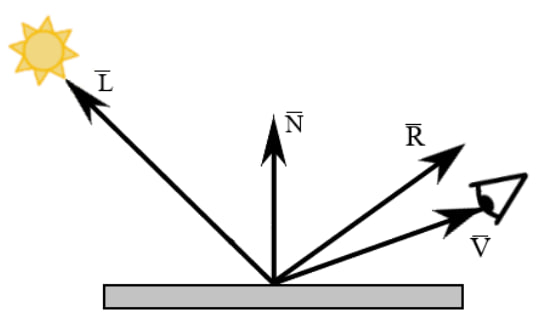
\includegraphics[width=.5\textwidth]{fong.jpg}
    \caption{Модель освещения Фонга}
    \label{fig:fong}
\end{figure}

На этом рисунке:
\begin{itemize}
    \item $\vec{L}$ --- вектор от точки на поверхности до источника света;
    \item $\vec{N}$ --- вектор нормали к поверхности в данной точке; 
    \item $\vec{R}$ --- вектор отражённого света;
    \item $\vec{V}$ --- вектор от точки на поверхности до наблюдателя (камеры);
\end{itemize}

Тогда интенсивность пикселя, отображающего данную точку на экране будет вычисляться согласно уравнению~\ref{eq:intens}.

\begin{equation}
    I = I_p \cdot K_a + I_0 \cdot K_b \cdot cos(\vec{L}, \vec{N}) + I_0 \cdot K_c \cdot cos^\alpha(\vec{R}, \vec{V})  
    \label{eq:intens}
\end{equation}

где $I$~---~итоговая интенсивность пикселя, отображающего данную точку на экране, $I_p$~---~интенсивность рассеянного света, $I_0$~---~интенсивность источника света, $K_a, K_b, K_c$~---~коэффициенты рассеянного, диффузного и зеркального освещения соответственно, $\alpha$~---~коэффициент блеска. 

$K_a, K_b, K_c, \alpha$ являются параметрами поверхности и, соответственно, константами. 

$I_p, K_a$ --- параметры модели освещения и тоже являются константами.

\subsection{Модель с картами освещения}

Модель с картами освещения --- это метод ускорить вычисления интенсивности освещения путём вычисления большинства параметров в момент построения сцены~\cite{LightMaps}. Такая модель может работать только в сценах, где положение объектов и источника(ов) освещения статичны. Сам метод сильно похож на метод теневых карт, однако вместо сохранения освещённости области изображения, будут сохранены значения векторов падающих на поверхность (и отражённых) лучей. 

Этот метод можно использовать вместе с моделью Фонга, чтобы значительно ускорить визуализацию очередного кадра.

Карту освещения, как и карту теней, придётся рассчитывать заново только если переместится источник света. В этот момент можно будет рассчитать все слагаемые из формулы~\ref{eq:intens} кроме последнего, а в последнем слагаемом останется рассчитать лишь косинус угла между векторами.

\subsection{Вывод}

В этой работе я буду использовать модель освещения Фонга с ускорением, использующим метод карт освещения. Поскольку построение реалистичного изображения не является целью работы, использовать более сложные (глобальные) модели освещения не нужно.

\clearpage

\chapter{Конструкторская часть}

\section{Требования к программному обеспечению}

Программа должна предоставлять графический интерфейс со следующим функционалом:
\begin{itemize}
    \item задавать параметры генерации модели загородного посёлка и генерировать его;
    \item изменять положение источника света;
    \item изменять положение и направление камеры.
\end{itemize}

Программа должна соответствовать следующим требованиям:
\begin{itemize}
    \item генерация (или конструирование) посёлка происходит при нажатии на соответствующую кнопку в интерфейсе;
    \item генерация осуществляется в соответствии с параметрами, заданными пользователем;
    \item программа должна корректно обрабатывать ввод некорректных данных.
\end{itemize}


\section{Описание структур данных}

\subsection*{Структуры данных, описывающие содержимое сцены}

\begin{enumerate}
    \item Сцена представляет собой список, содержащий указатели на объекты сцены (дома, дороги и т.п.);
    \item Объекты сцены включают в себя следующие данные:\begin{itemize}
        \item массив поверхностей;
        \item матрица преобразований.
    \end{itemize}
    \item Поверхность включает в себя следующие данные: \begin{itemize}
        \item массив вершин;
        \item вектор нормали;
        \item спектральные характеристики.
    \end{itemize}
    \item Вершины включают в себя следующие данные: \begin{itemize}
        \item координаты вершины.
    \end{itemize}
    \item Источник света включает в себя следующие данные: \begin{itemize}
        \item координаты источника.
    \end{itemize}
    \item Камера включает в себя следующие данные: \begin{itemize}
        \item координаты камеры; 
        \item матрица преобразований направления камеры.
    \end{itemize}
\end{enumerate}

Следует отметить, что матрица преобразований камеры описывает как её координаты, так и её направление. 

Камера с единичной матрицей трансформации находится в точке с координатами $(0,0,0)$ и направлена вдоль оси $X$.

\subsection*{Структуры данных, необходимые для генерации сцены}

В процессе генерации, содержимое сцены описывается матрицей (двумерным массивом), каждая ячейка которой означает нахождение определённого объекта на координатах, соответствующих данной ячейке матрицы.

Объекты матрицы содержат следующие данные:
\begin{itemize}
    \item идентификатор типа объекта;
    \item таблица возможных идентификаторов типов соседних клеток (по одной записи на каждую соседнюю ячейку).
\end{itemize}


\section{Алгоритм построения изображения}

К алгоритму построения алгоритма приведены следующие требования:
\begin{itemize}
    \item на вход подаётся список объектов сцены, описание источника света и камеры;
    \item на выход подаётся построенное изображение.
\end{itemize}

Алгоритм построения изображения представлен на рисунке~\ref{fig:rendering}.

\begin{figure}[h!]
    \centering
    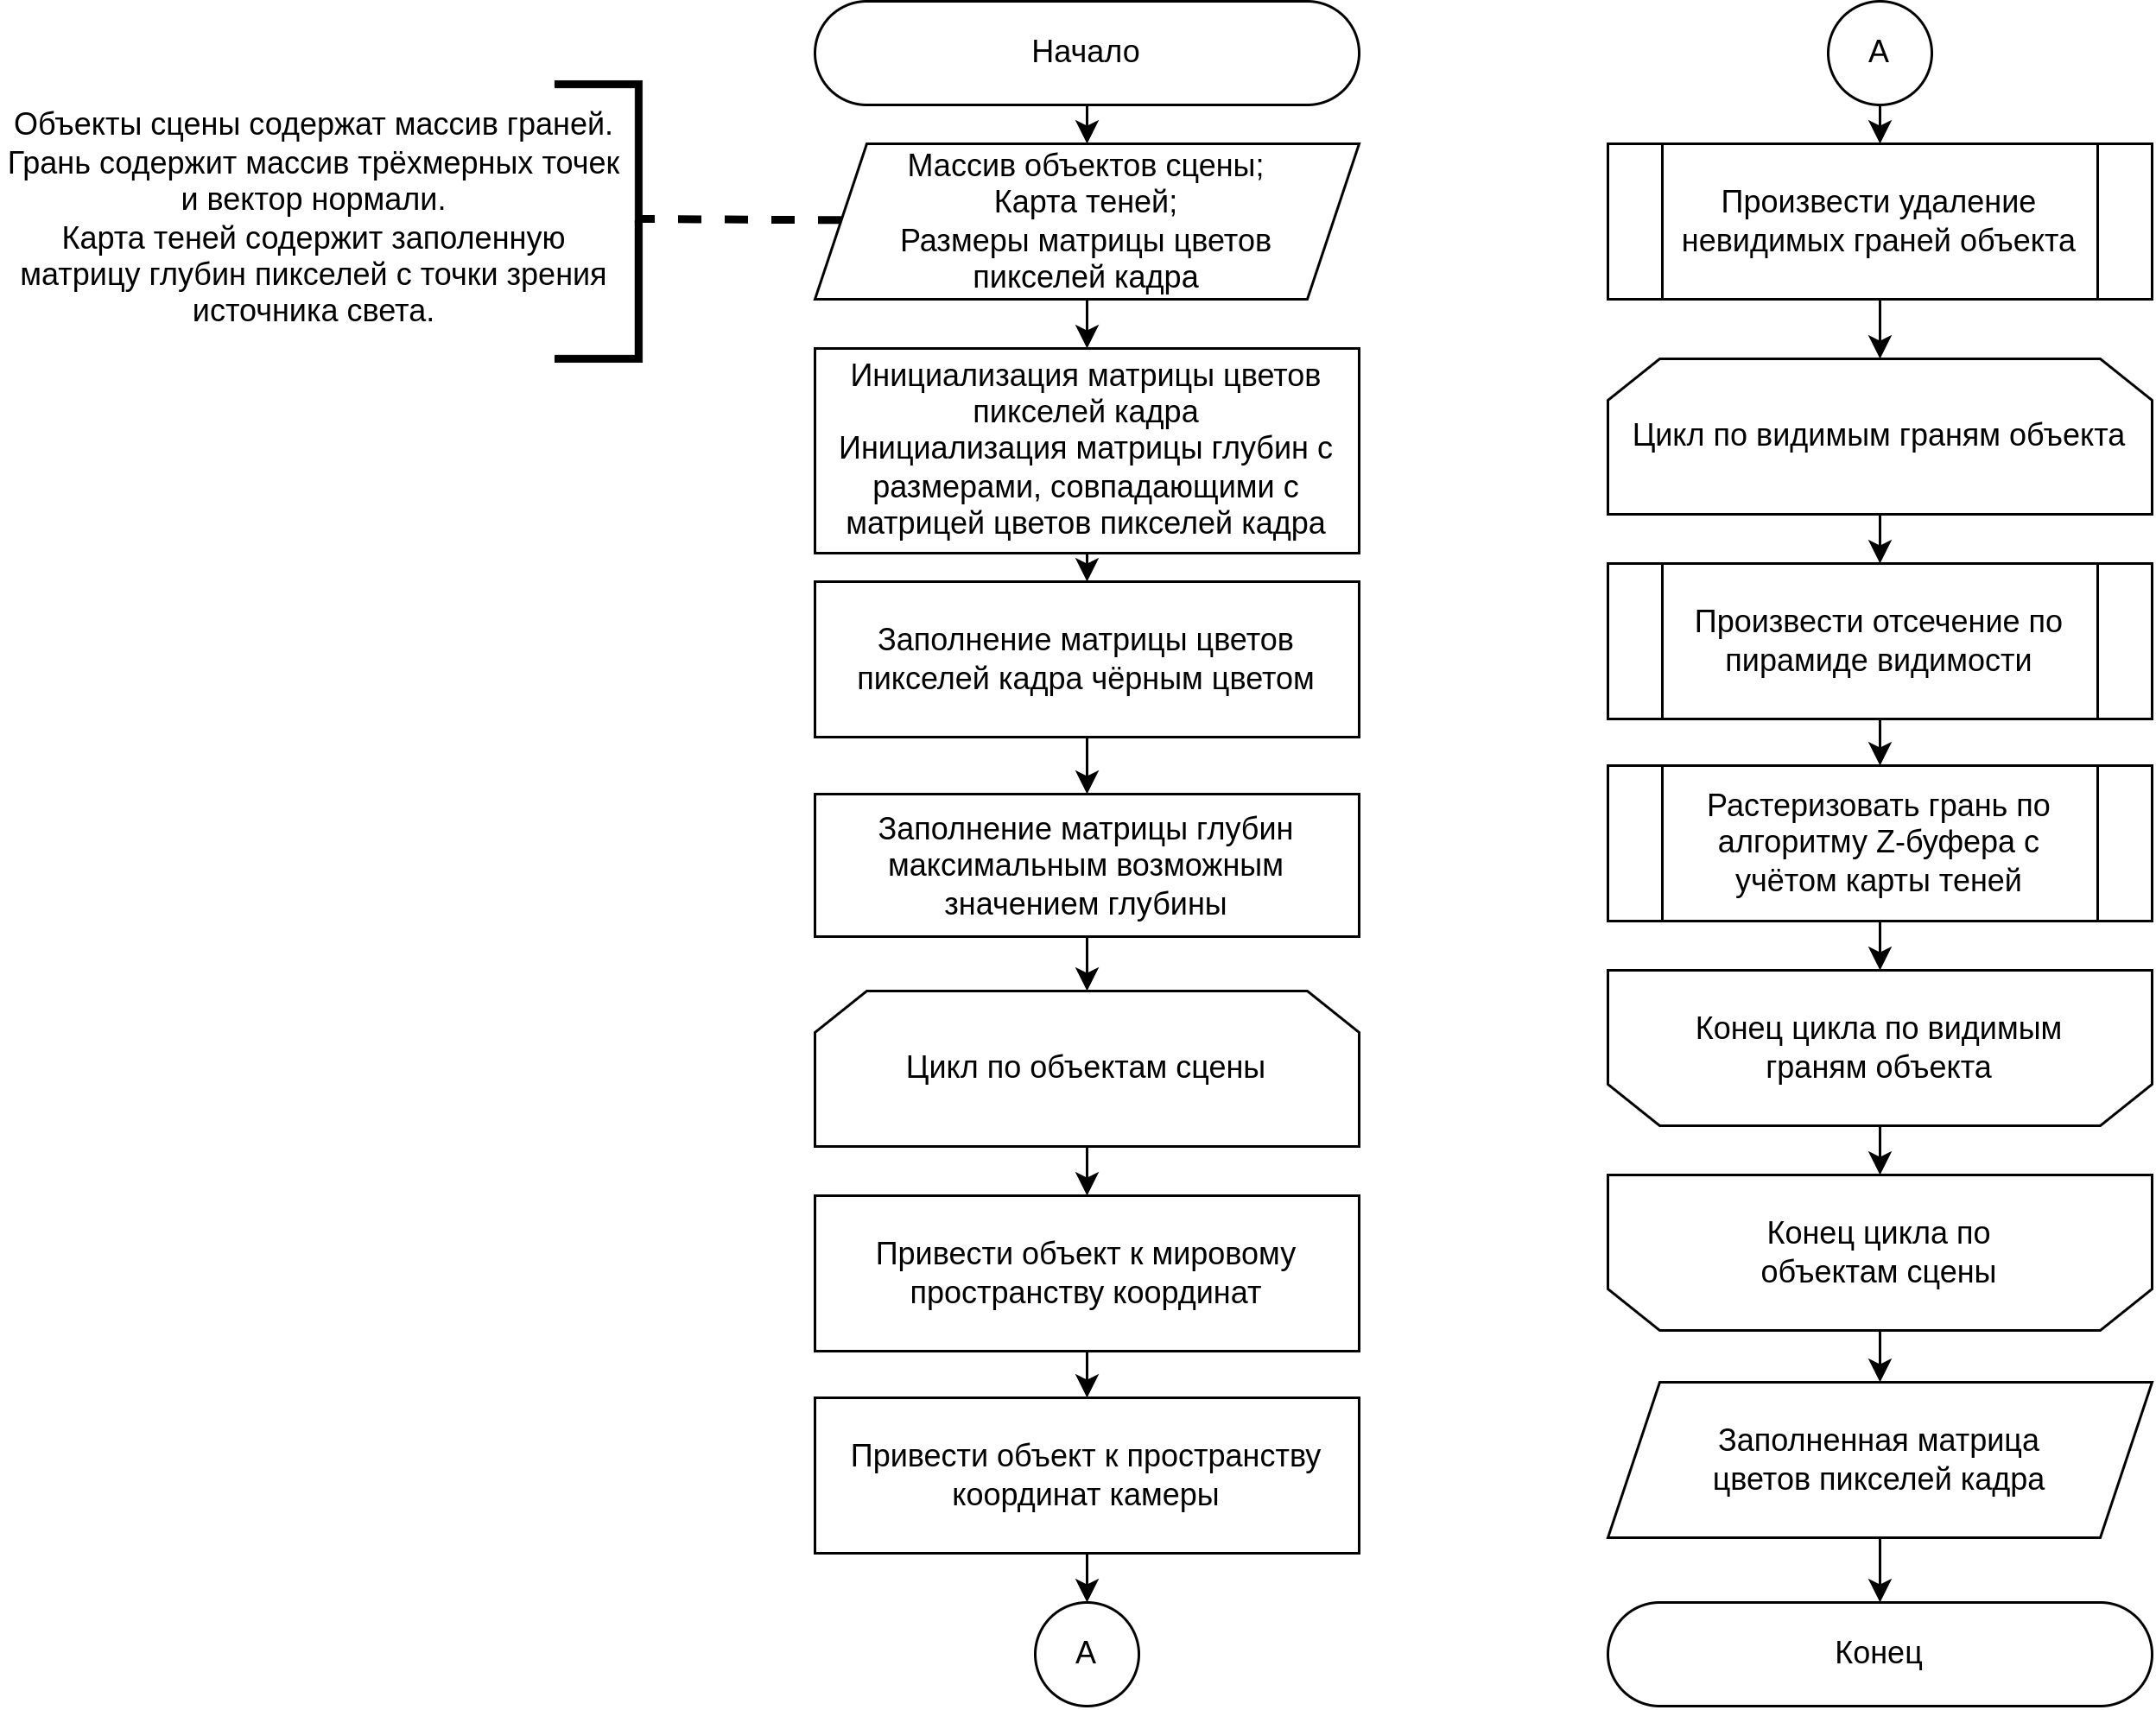
\includegraphics[width=.5\textwidth]{rendering.drawio.png}
    \caption{Алгоритм построения изображения}
    \label{fig:rendering}
\end{figure}

В следующих пунктах будут подробнее описаны этапы данного алгоритма.

\subsection{Матрицы преобразования}

В данном алгоритме (и структурах данных) под словосочетанием ``матрица преобразования'' подразумеваются такая матрица, при умножении всех точек объекта на которую, будет получен преобразованный объект~\cite{CGPaP}.

Данная матрица, как правило, получается как результат произведения нескольких матриц аффинных преобразований.

В данной работе используются следующие аффинные преобразования:

\begin{itemize}
    \item перенос;
    \item масштабирование;
    \item поворот.
\end{itemize}

Матрица переноса представляется следующим образом:
$$
\begin{pmatrix}
    1 & 0 & 0 & 0 \\
    0 & 1 & 0 & 0 \\
    0 & 0 & 1 & 0 \\
    dx & dy & dz & 1
\end{pmatrix}
$$

здесь, $dx, dy, dz$ --- это смещения по осям $Ox, Oy$ и $Oz$ соответственно.

Матрица масштабирования представляется следующим образом:

$$
\begin{pmatrix}
    kx & 0 & 0 & 0 \\
    0 & ky & 0 & 0 \\
    0 & 0 & kz & 0 \\
    0 & 0 & 0 & 1
\end{pmatrix}
$$

здесь, $kx, ky, kz$ --- это коэффициенты масштабирования по осям $Ox, Oy$ и $Oz$ соответственно.

Матрицы поворота представляются по-разному для каждой оси.

Матрица поворота вокруг оси $Ox$ представляется следующим образом:

$$
\begin{pmatrix}
    1 & 0 & 0 & 0 \\
    0 & cos \alpha & sin \alpha & 0 \\
    0 & -sin \alpha & cos \alpha & 0 \\
    0 & 0 & 0 & 1
\end{pmatrix}
$$

Матрица поворота вокруг оси $Oy$ представляется следующим образом:

$$
\begin{pmatrix}
    cos \alpha & 0 & -sin \alpha & 0 \\
    0 & 1 & 0 & 0 \\
    sin \alpha & 0 & cos \alpha & 0 \\
    0 & 0 & 0 & 1
\end{pmatrix}
$$

Матрица поворота вокруг оси $Oz$ представляется следующим образом:

$$
\begin{pmatrix}
    cos \alpha & sin \alpha & 0 & 0 \\
    -sin \alpha & cos \alpha & 0 & 0 \\
    0 & 0 & 1 & 0 \\
    0 & 0 & 0 & 1
\end{pmatrix}
$$

Во всех матрицах вращения, $\alpha$ --- угол поворота вокруг соответствующей оси в радианах.

\subsection{Приведение к пространству камеры}

Поскольку положение и направление камеры описывается матрицей преобразований, приведение точки к пространству координат камеры равносильно применению к данной точке обратных преобразований, применённых к камере.

Например при смещении камеры на 10 точек по оси $Ox$, относительно камеры объекты сцены сместятся на -10 точек по той же оси. При повороте камеры на 10 градусов вокруг оси $Ox$, объекты сцены повернутся на -10 градусов вокруг той же оси относительно координат камеры.

Пользуясь этим свойством, для упрощения перевода координат точек в пространство камеры, можно воспользоваться следующим приёмом: при преобразовании камеры (координат и направления) можно записывать в её матрицу преобразования обратные значения.

Таким образом, для приведения точки к пространству камеры, достаточно применить к этой точке матрицу преобразования камеры.

% \subsection{Перспективная проекция}

Данная секция пока что вырезана, если вы это видите, значит у вас есть сорс и вы молодец.


\subsection{Удаление невидимых поверхностей}

Удаление невидимых поверхностей для этой работы будет проводиться по двум критериям:

\begin{itemize}
    \item скалярное произведение нормали поверхности и вектора направления камеры;
    \item попадание поверхности в пирамиду видимости камеры.
\end{itemize}

Первый критерий позволяет удалить нелицевые (с точки зрения камеры) поверхности. Это позволяет существенно уменьшить количество поверхностей, которые придётся обрабатывать при построении буфера кадра.

Для определения видимости поверхности, достаточно вычислить значения скалярного произведения $(\vec{N}, \vec{V})$, где $\vec{N}$ --- вектор нормали поверхности, а $\vec{V}$ --- вектор направления камеры. Тогда, при значении $(\vec{N}, \vec{V})$ меньшем нулю, поверхность будет лицевой, а во всех остальных случаях - нелицевой.

Следует отметить, что для правильного определения нелицевых граней, их необходимо также переводить в пространство перспективной проекции, если таковое используется при построении сцены.

Второй критерий позволяет удалить те поверхности которые не попадают в поле зрения камеры. Часто для упрощения вычислений этого критерия, используется не сама поверхность (которая может задаваться сложной фигурой), а параллелепипед, вписывающий данную поверхность в себя.

Удобно использовать такой параллелепипед, стороны которого параллельны осям системы координат камеры. Тогда, для вычисления его параметров будет достаточно вычислить максимальные и минимальные значения каждой из координат.

После этого, выполняется определение видимость этого параллелепипеда путём пересечения его с пирамидой видимости камеры~\cite{Rogers}.

Определение пересечения бесконечной пирамиды и прямоугольника тривиально, и сводится к определению определению пересечения прямых.  

\subsection{Алгоритм Z-буфера}



\subsection{Построение теней}

Как и упоминалось в аналитической части, карта теней представляет из себя совокупность матрицы преобразования координат в пространство координат источника света и матрицы глубин, вычисленной с точки зрения источника света. 

Вычисление матрицы глубин для карты теней использует упрощённую версию алгоритма с рисунка~\ref{fig:z-buffer}. Отличие заключается в том, что для карты теней не нужно заполнять матрицу цветов пикселей кадра. На вход поступают точки многоугольника, приведённые в пространство координат источника света. Вместо пространства координат экрана, используется пространство координат карты теней, которое использует ортогональную проекцию вместо перспективной.

Таким образом, алгоритм заполнения матрицы глубин для одного многоугольника изображён на рисунке~\ref{fig:smap_buffer}.

\begin{figure}[h!]
  \centering
  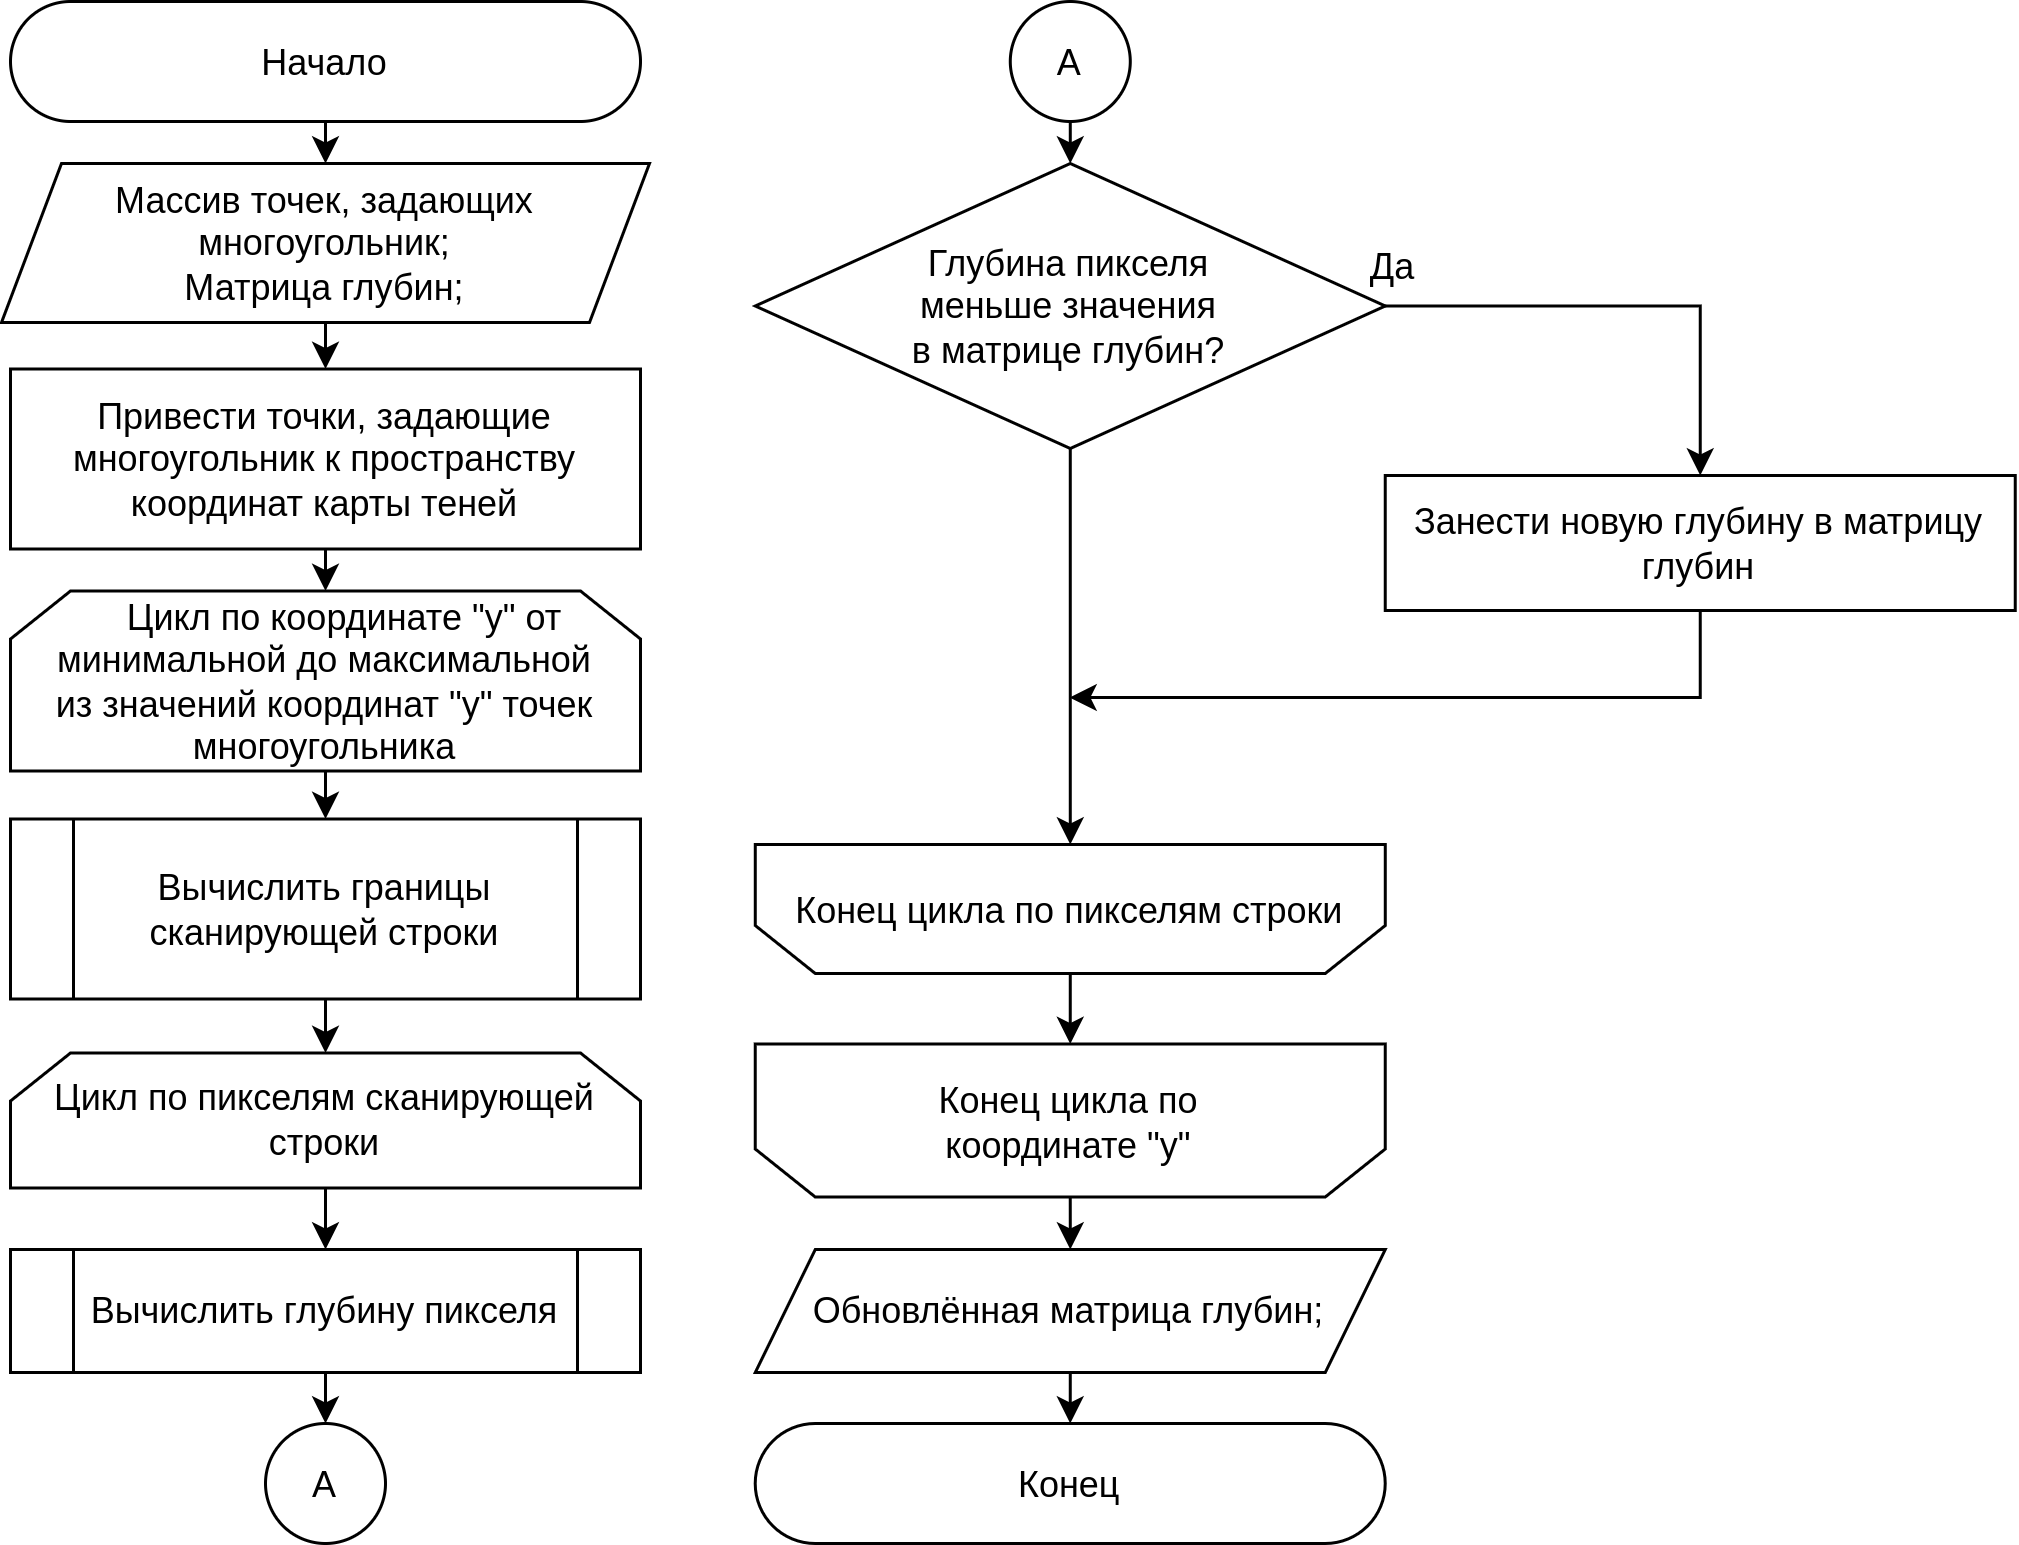
\includegraphics[height=.5\textheight]{smap.drawio.png}
  \caption{Алгоритм заполнения матрицы глубин для одного многоугольника}
  \label{fig:smap_buffer}
\end{figure}

Для вычисления цвета пикселя, находящегося в тени, используется формула~\eqref{eq:shadow}:

\begin{equation}
  \label{eq:shadow}
  \begin{split}
    r_1 = r*p \\
    g_1 = g*p \\ 
    b_1 = b*p
  \end{split}
  \end{equation}

, где $r_1, g_1, b_1$ --- значения интенсивности красного, зелёного и синего каналов цвета пикселя после затенения соответственно; $p$ --- коэффициент затенения; $r, g, b$ --- значения интенсивности красного, зелёного и синего каналов цвета исходного пикселя соответственно.

В данной работе был выбран коэффициент затенеия $p = 0.4$.




\section{Алгоритм генерации сцены}

Для генерации сцены будет использован алгоритм квантового коллапса волновой функции. 

Для корректной работы алгоритма крайне важно правильное задание начальных ограничений. Под ограничением подразумевается возможность или невозможность появления определённого состояния ячейки вплотную к другому состоянию ячейки с определённой стороны~\cite{QWFC}.

Например если в одной ячейке содержится состояние, представляющее прямой участок дороги, то к тем сторонам ячейки, которые пересекает дорога, могут быть ``присоединены'' ячейки с только такими состояниями, в которых к этим же сторонам будут присоединены другие участки дороги. Это ограничение изображено на рисунке~\ref{fig:restrictions}.

\begin{figure}[h!]
    \centering
    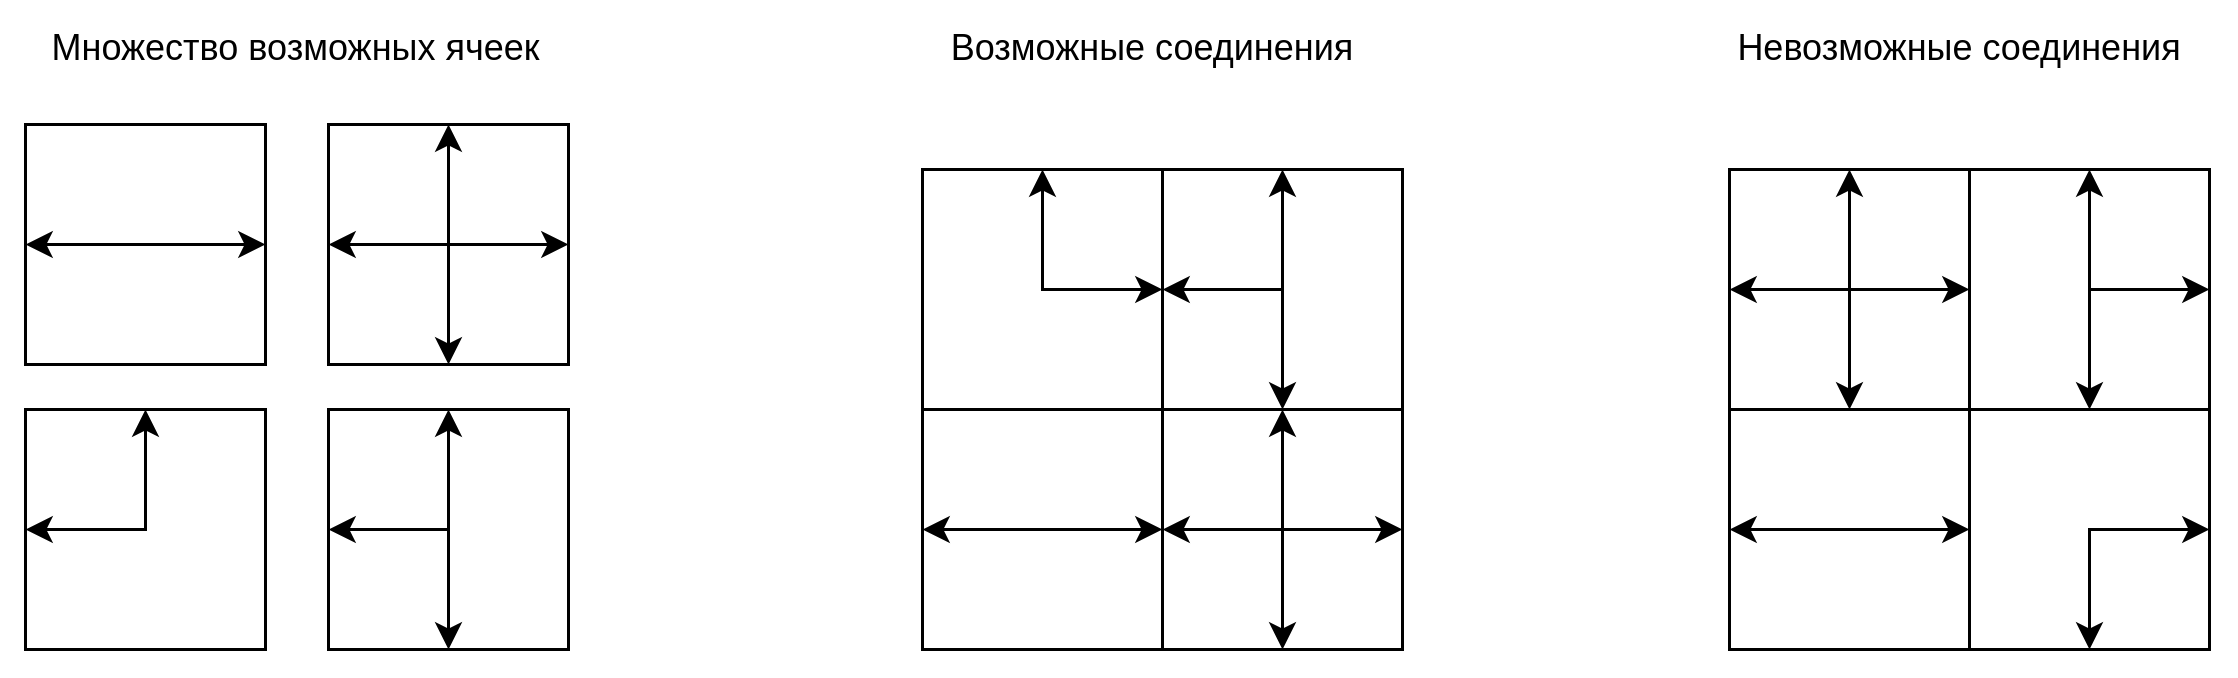
\includegraphics[width=.9\textwidth]{restrictions.drawio.png}
    \caption{Визуализация ограничений генерации}
    \label{fig:restrictions}
\end{figure}

Описание ограничений выполняется вручную для каждого возможного состояния ячейки.

Пусть необходимо заполнить матрицу генерации $M$ размером 50 на 50 ячеек. Изначально все ячейки находятся в состоянии суперпозиции, то есть каждая ячейка может принять любое возможное состояние. Возможные состояния, в свою очередь, определяются пересечением ограничений соседних ячеек. Если какой-либо из соседей не находится в строго определённом состоянии, его ограничениями будет являться объединение ограничений каждого из его возможных состояний.

Пока все ячейки матрицы не примут строго определённое состояние, выполняется цикл, который выбирает ячейку с наименьшим количеством возможных состояний и фиксирует её значение, выбирая случайным образом одно из возможных состояний.

Предусмотрена возможность повлиять на вероятность выбора того или иного состояния ячейки путём задания некоторого приоритета. Например, в случае с дорогами, можно повысить вероятность появления поворота и уменьшить вероятность появления перекрёстка.

После обновления ячейки в матрице, возможные состояния её соседних ячеек обновляются.

Алгоритм коллапса волновой функции представлен на рисунке~\ref{fig:QWFC}.

\newpage

\begin{figure}[h!]
    \centering
    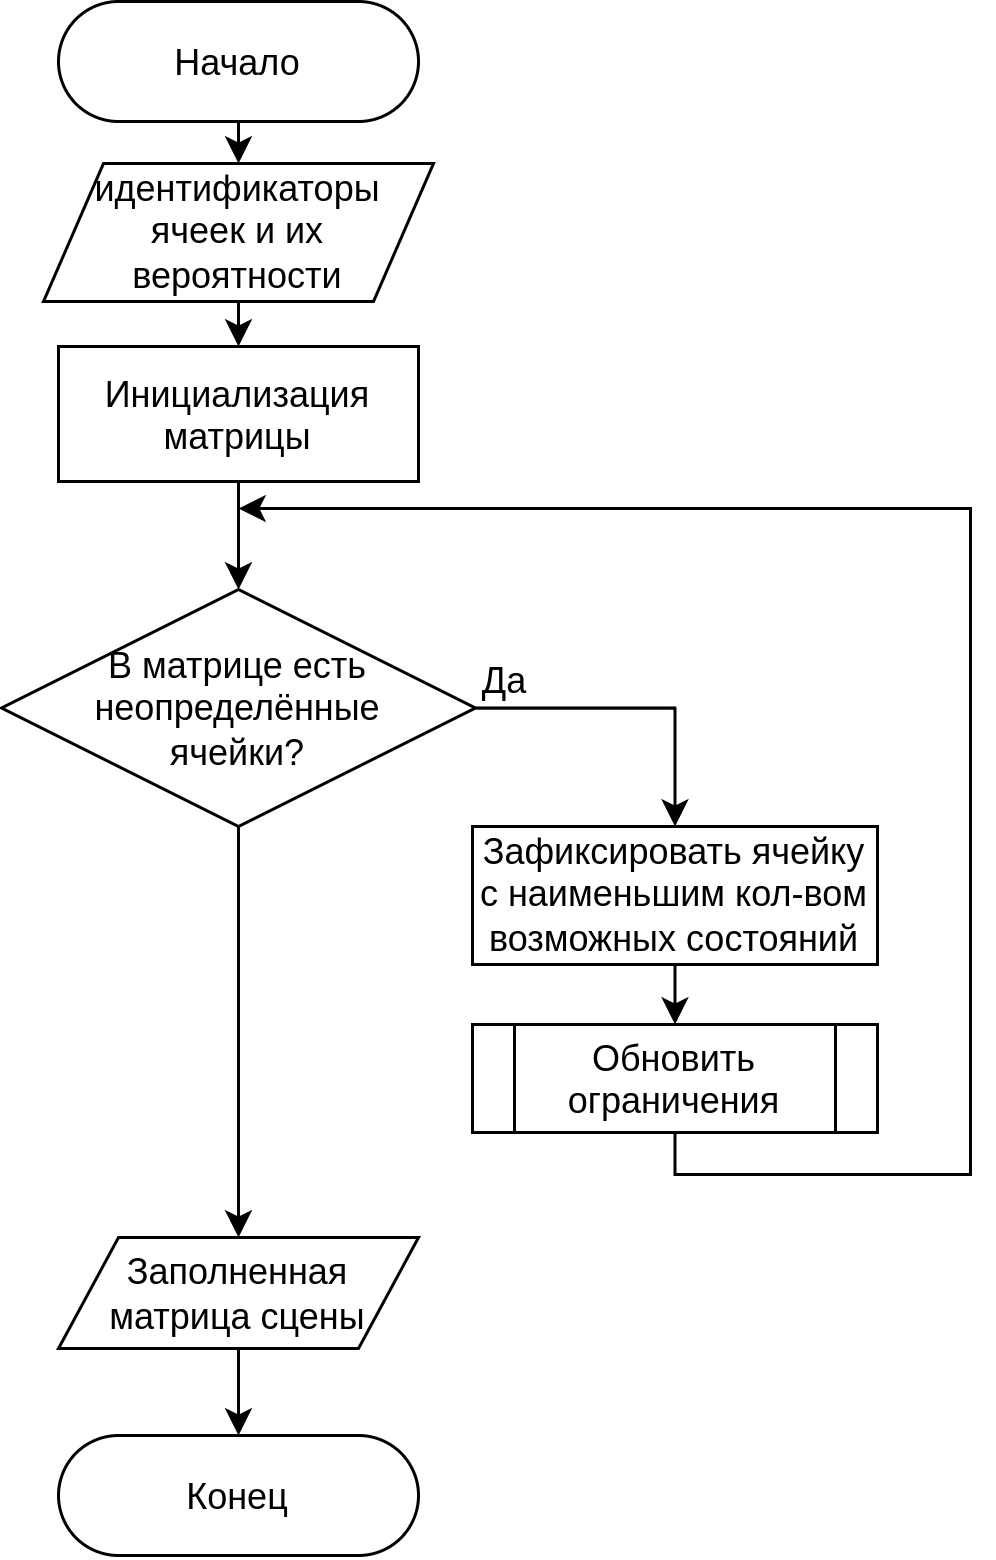
\includegraphics[width=.8\textwidth]{QWFC.drawio.png}
    \caption{Алгоритм квантового коллапса волновой функции}
    \label{fig:QWFC}
\end{figure}

В рамках данной работы будут использованы 10 возможных состояний ячеек:

\begin{itemize}
    \item дорожный перекрёсток;
    \item горизонтальный прямой участок дороги;
    \item вертикальный прямой участок дороги;
    \item 4 типа угловых участков дороги;
    \item пустырь;
    \item дерево;
    \item дом.
\end{itemize}

Поскольку состояний ячеек для описания разных типов дорог семь, а для остальных типов объектов --- всего три, необходимо снизить вероятность появления каждого определённого типа дороги в семь раз. Такое снижение вероятности сравняло бы шансы появления дороги или другого типа объекта в той или иной ячейке матрицы, однако вероятности дорог снижены неравномерно для уменьшения количества перекрёстков и поворотов.

Таким образом, получаем скорректированные вероятности появления:
\begin{itemize}
    \item перекрёстка --- 10\%;
    \item прямых участков --- 25\%;
    \item угловых участков --- 10\%.
\end{itemize}

Соотношение других типов объектов (и дорог) друг к другу также можно корректировать в интерфейсе приложения.



\chapter{Технологическая часть}

\section{Средства реализации}

\subsection*{Язык программирования}

Для реализации ПО был выбран язык программирования C++~\cite{cpp} стандарта ``C++20'' по следующим причинам:
\begin{itemize}
  \item данный язык является объектно-ориентированным, что позволяет проектировать сложные системы взаимодействия объектов для обработки и визуализации;
  \item стандартная библиотека языка достаточна для осуществления всех спроектированных алгоритмов;
  \item стандартная библиотека языка предоставляет средства для профилирования и исследования временных затрат;
  \item для языка разработано большое количество библиотек, расширяющих возможности языка. 
\end{itemize}

В процессе разработки ПО были использованы внешние библиотеки:
\begin{itemize}
  \item Qt6~\cite{qt} для осуществления интерфейса программы;
  \item OneApi TBB~\cite{tbb} для параллелизации процессов.
\end{itemize}

\subsection*{Система сборки}

В качестве системы сборки проекта была выбрана система CMake~\cite{CMake}, так как она предназначена для работы с языками C и C++ и предоставляет возможность контроля над подключаемыми файлами и библиотеками.

\subsection*{Среда разработки}

Для разработки была выбрана Visual Studio Code~\cite{vscode}, так как она предоставляет достаточный интерфейс для написания и отладки кода, а также обеспечивает возможность работы с избранной системой сборки.

Для редактирования интерфейса была использована программа QtDesigner, поставляемая вместе с библиотекой Qt.

\section{Структура классов}

Были разработаны следующие классы:
\begin{itemize}
  \item \emph{Point2D} --- для работы с точками на плоскости;
  \item \emph{Point3D} --- для работы с точками в пространстве;
  \item \emph{Triangle} --- для работы с треугольниками в пространстве;
  \item \emph{Plane} --- для работы с плоскостями;
  \item \emph{Color} --- описывающий цвет;
  \item \emph{Face} --- для работы с гранями объектов;
  \item \emph{Square} --- класс, описывающий квадрат в пространстве;
  \item \emph{Cube} --- класс, описывающий куб в пространстве;
  \item \emph{BaseModel} --- базовый класс модели на сцене;
  \item \emph{FaceModel} --- класс для работы с поверхностными моделями;
  \item \emph{House} --- класс, описывающий модель дома;
  \item \emph{Tree} --- класс, описывающий модель дерева;
  \item \emph{RoadXX} --- классы, описывающие модели дорог разных видов;
  \item \emph{TransformationMatrix} --- класс, описывающий матрицу трансформации моделей;
  \item \emph{Scene} --- класс, хранящий объекты сцены;
  \item \emph{BaseCamera} --- базовый класс, описывающий камеры;
  \item \emph{PerspectiveCamera} --- камера, отображающая точки по принципу перспективной проекции;
  \item \emph{ShadowMap} --- класс, предоставляющий доступ к карте теней;
  \item \emph{BaseVisitor} --- базовый класс для паттерна программирования ``посетитель'';
  \item \emph{ShadowMapVisitor} --- ``посетитель'', производящий вычисление карты теней;
  \item \emph{RenderVisitor} --- ``посетитель'', производящий вычисление матрицы цветов кадра;
  \item \emph{QWFC} --- класс, осуществляющий генерацию матрицы сцены;
  \item \emph{Cell} --- класс, описывающий ячейку для алгоритма QWFC;
  \item \emph{Rule} --- класс, описывающий правило для алгоритма QWFC.
\end{itemize}

Схема разработанных классов изображена на рисунке~\ref{fig:UML}.

\begin{figure}[h]
  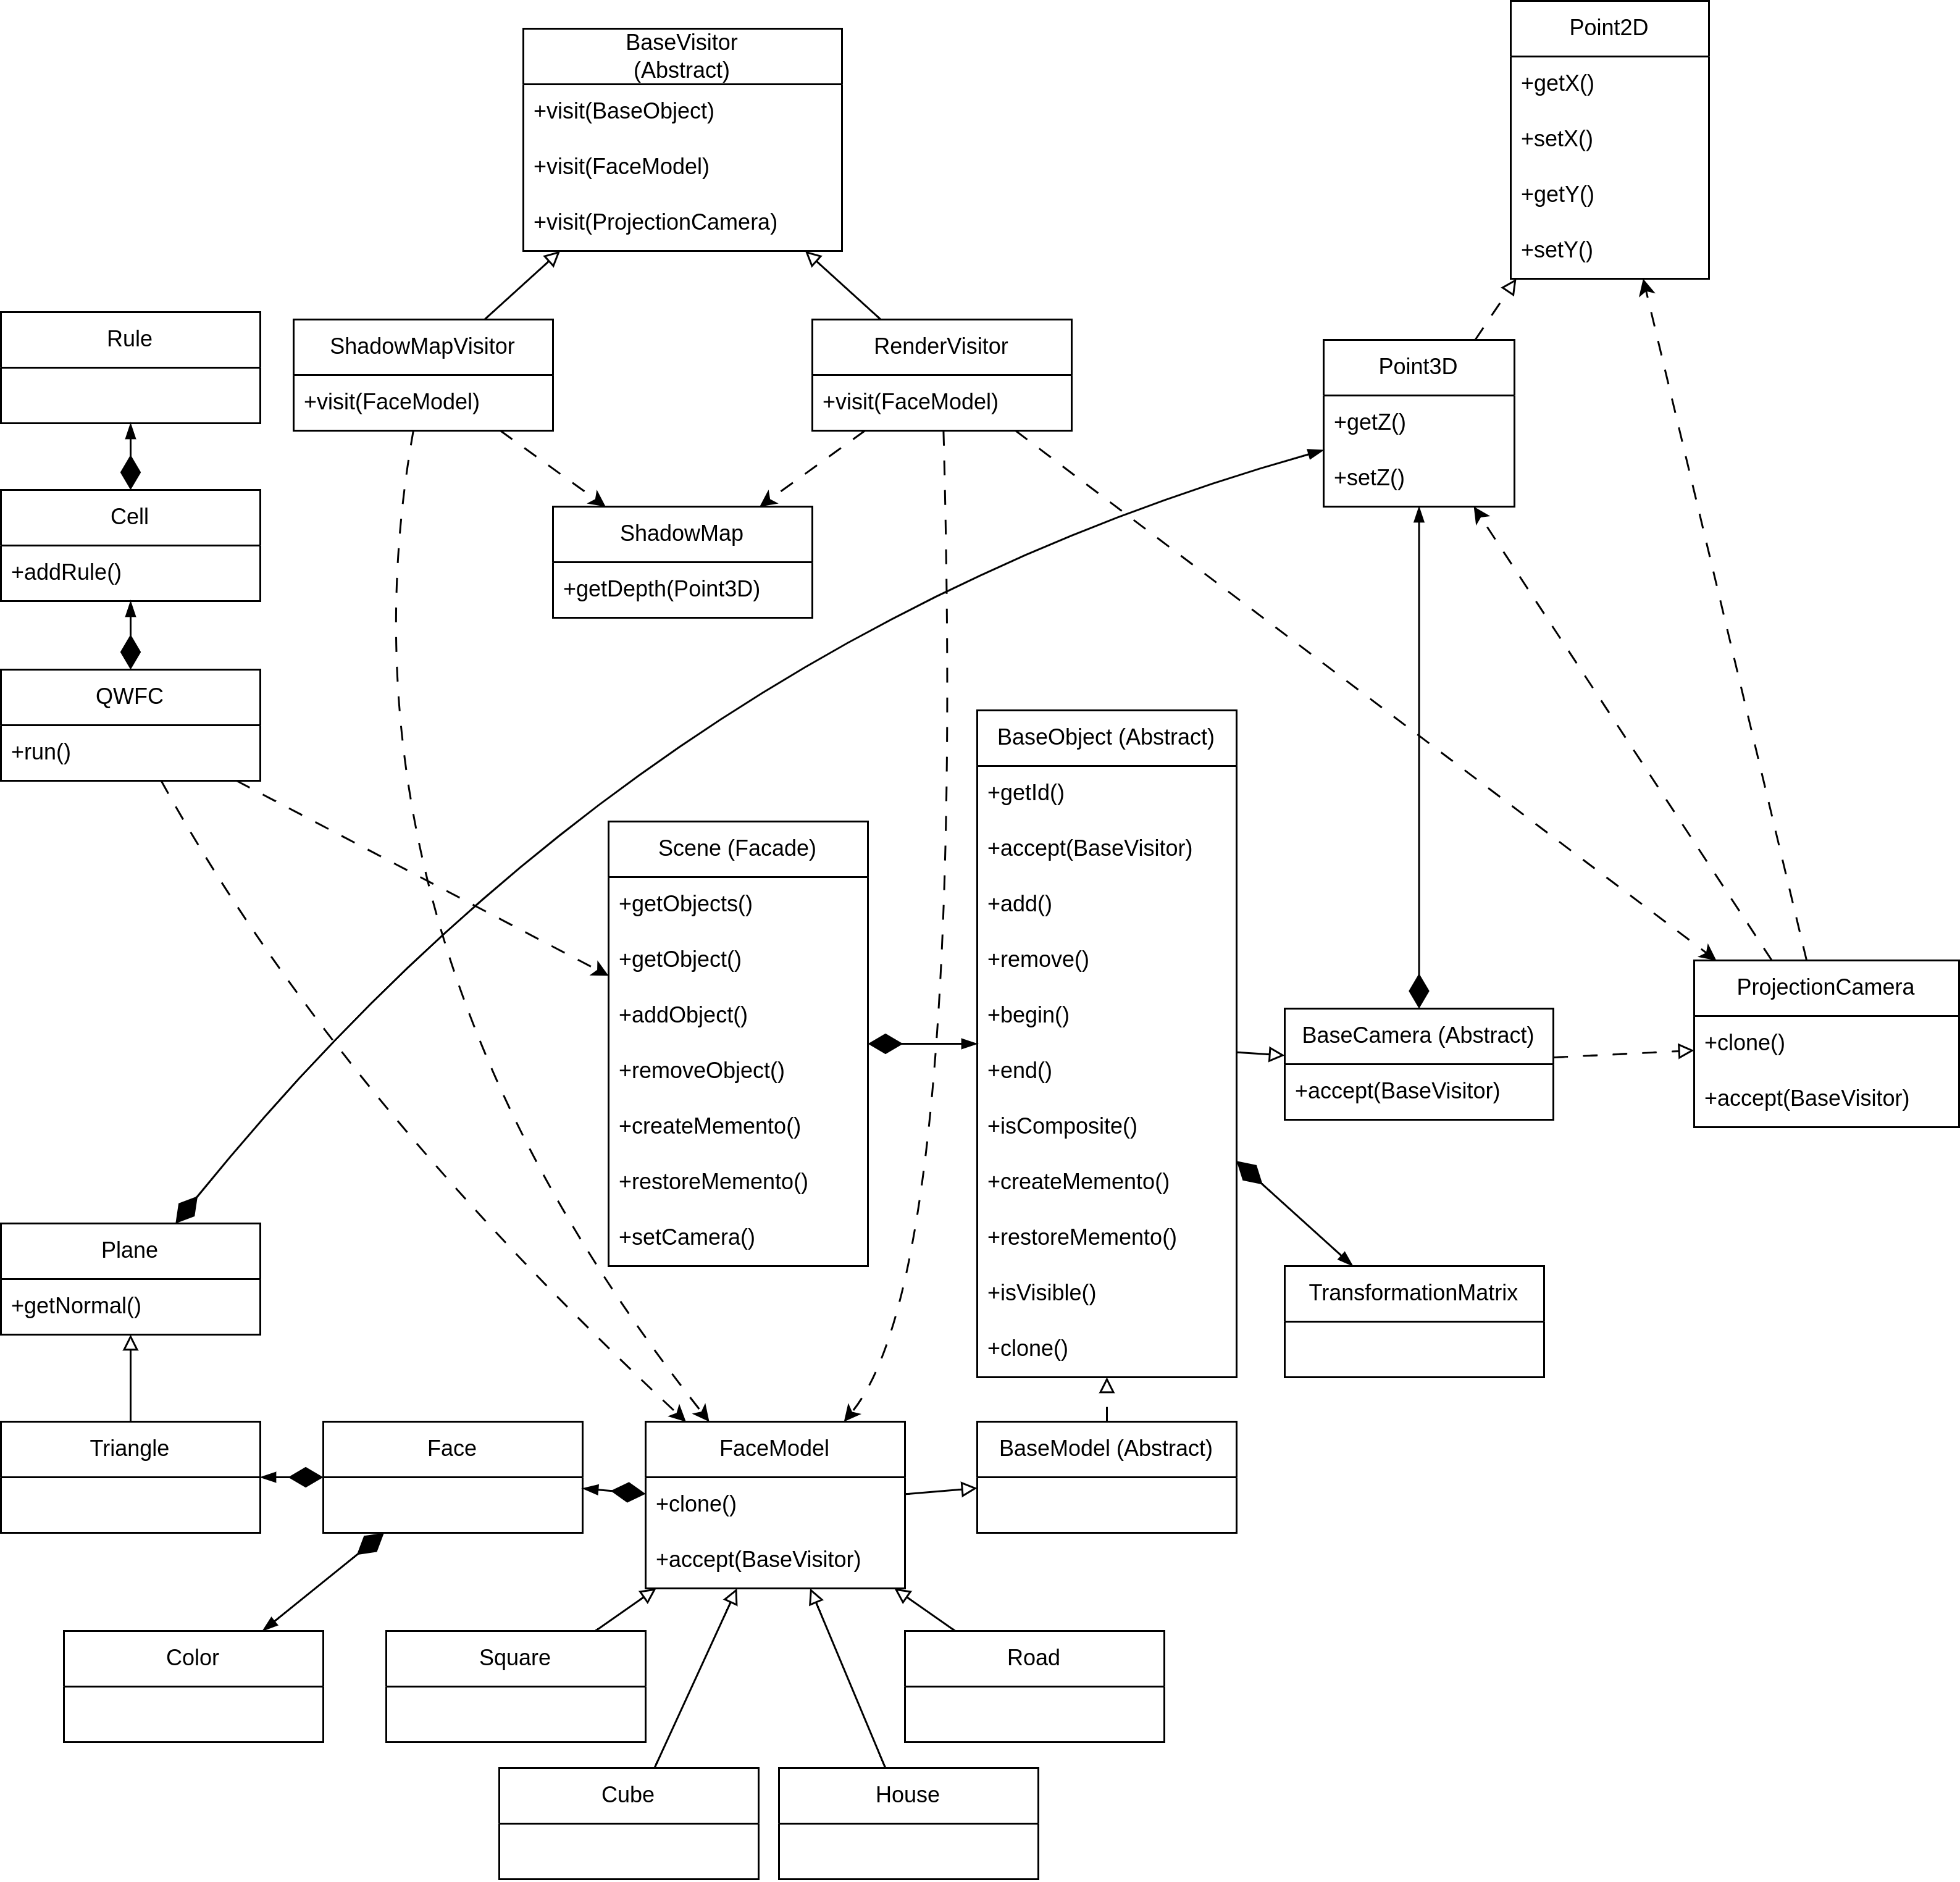
\includegraphics[width=\textwidth]{diagram.drawio.png}
  \caption{Диаграмма классов}
  \label{fig:UML}
\end{figure}

Из перечисления выше исключены те классы и структуры, которые используются только для связи с интерфейсом и библиотекой Qt во избежание загромождения.

\section{Реализация ПО}

Процесс отрисовки изображения с помощью алгоритма Z-буфера происходит при использовании класса RenderVisitor на сцену. 
Эта функция представлена на листинге~\ref{lst:render_scene}. 

На этом этапе происходит инициализация матрицы глубин и матрицы цветов пикселей кадра. Затем RenderVisitor обрабатывает каждый объект на сцене. Этот процесс происходит с использованием библиотеки tbb, поэтому каждый объект обрабатывается параллельно, что позволяет сильно сократить время создания кадра (см. исследовательскую часть).

Поскольку алгоритм Z-буфера не рассчитан на одновременную обработку несколькими потоками, для каждого объекта сцены создаётся набор заполненных матриц глубин и матриц цветов пикселей кадра --- по одному для каждой видимой грани объекта. 
Эти промежуточные матрицы объединяются в однопоточном виде для получения итоговой матрицы цветов пикселей кадра.

Функция обработки модели объектом RenderVisitor представлена на листинге~\ref{lst:render_model}.

Из каждого объекта извлекаются грани, затем происходит фильтрация невидимых граней алгоритмами отсечения невидимых поверхностей. Оставшиеся грани создают матрицы глубин и цветов пикселей кадра, а затем сохраняют их в общий массив. 

Обработка каждой грани также происходит одновременно. 

Поскольку все грани в моей работе представляются треугольниками, процесс растеризации был оптимизирован для них.

Координаты глубины и мировых координат вычисляются итерационно для каждой сканирующей строки треугольника в соответствии с алгоритмом, разработанным в аналитической части.
Также в этом методе происходит сравнение координат точек с координатами в карте теней.

Вычисление карты теней выполняется аналогично заполнению матрицы глубин для основного кадра, но вместо матрицы преобразования в пространство координат камеры, используется матрица преобразования в пространство координат источника света.

Заполнение матрицы цветов пикселей кадра происходит каждый раз когда изменяется сцена, то есть меняется положение и/или направление камеры, изменяется положение источника света или изменяются объекты на сцене.

Расчёт карты теней происходит только при изменении положения источника света или изменении объектов на сцене.

Метод collapseCell класса QWFC представлен на листинге~\ref{lst:qwfcoll}. Фиксирование состояния ячейки производится в соответствии с приоритетами, их учёт можно увидеть в этой функции.

После фиксирования состояния ячейки состояние соседних ячеек рекурсивно обновляется.

Для тестирования алгоритма QWFC, вместе с основным файлом программы ``app'', собирается файл ``qwf'', производящий замеры времени генерации сцены.

\section*{Пользовательский интерфейс}

Пользовательский интерфейс состоит из описанных ниже групп управления.

\subsection*{Группа управления генерацией сцены}

В данной группе управления пользователю доступны:
\begin{itemize}
  \item два поля ввода для задания размеров матрицы сцены;
  \item четыре поля ввода для задания вероятностей появления разных типов объектов;
  \item кнопка ``создать'', осуществляющая генерацию новой сцены.
\end{itemize}

\subsection*{Группа управления положения источника света}

В данной группе управления пользователю доступны два ползунка для управления поворотом источника вокруг осей $Ox$ и $Oy$.

Управление камерой производится с помощью клавиатуры:
\begin{itemize}
  \item клавиши ``W'', ``A'', ``S'', ``D'' используются для движения камеры вперёд, влево, назад и вправо соответственно;
  \item клавиши ``I'', ``J'', ``K'', ``L'' используются для поворотов камеры вверх, влево, вниз и вправо соответственно;
  \item клавиши ``Пробел'' и ``B'' используются для движения камеры вверх и вниз вдоль оси $Oy$ соответственно.
\end{itemize}



\section{Демонстрация работы программы}

На рисунках~\ref{fig:example_1}-\ref{fig:example_5} представлены примеры работы программы.

\begin{figure}[h!]
  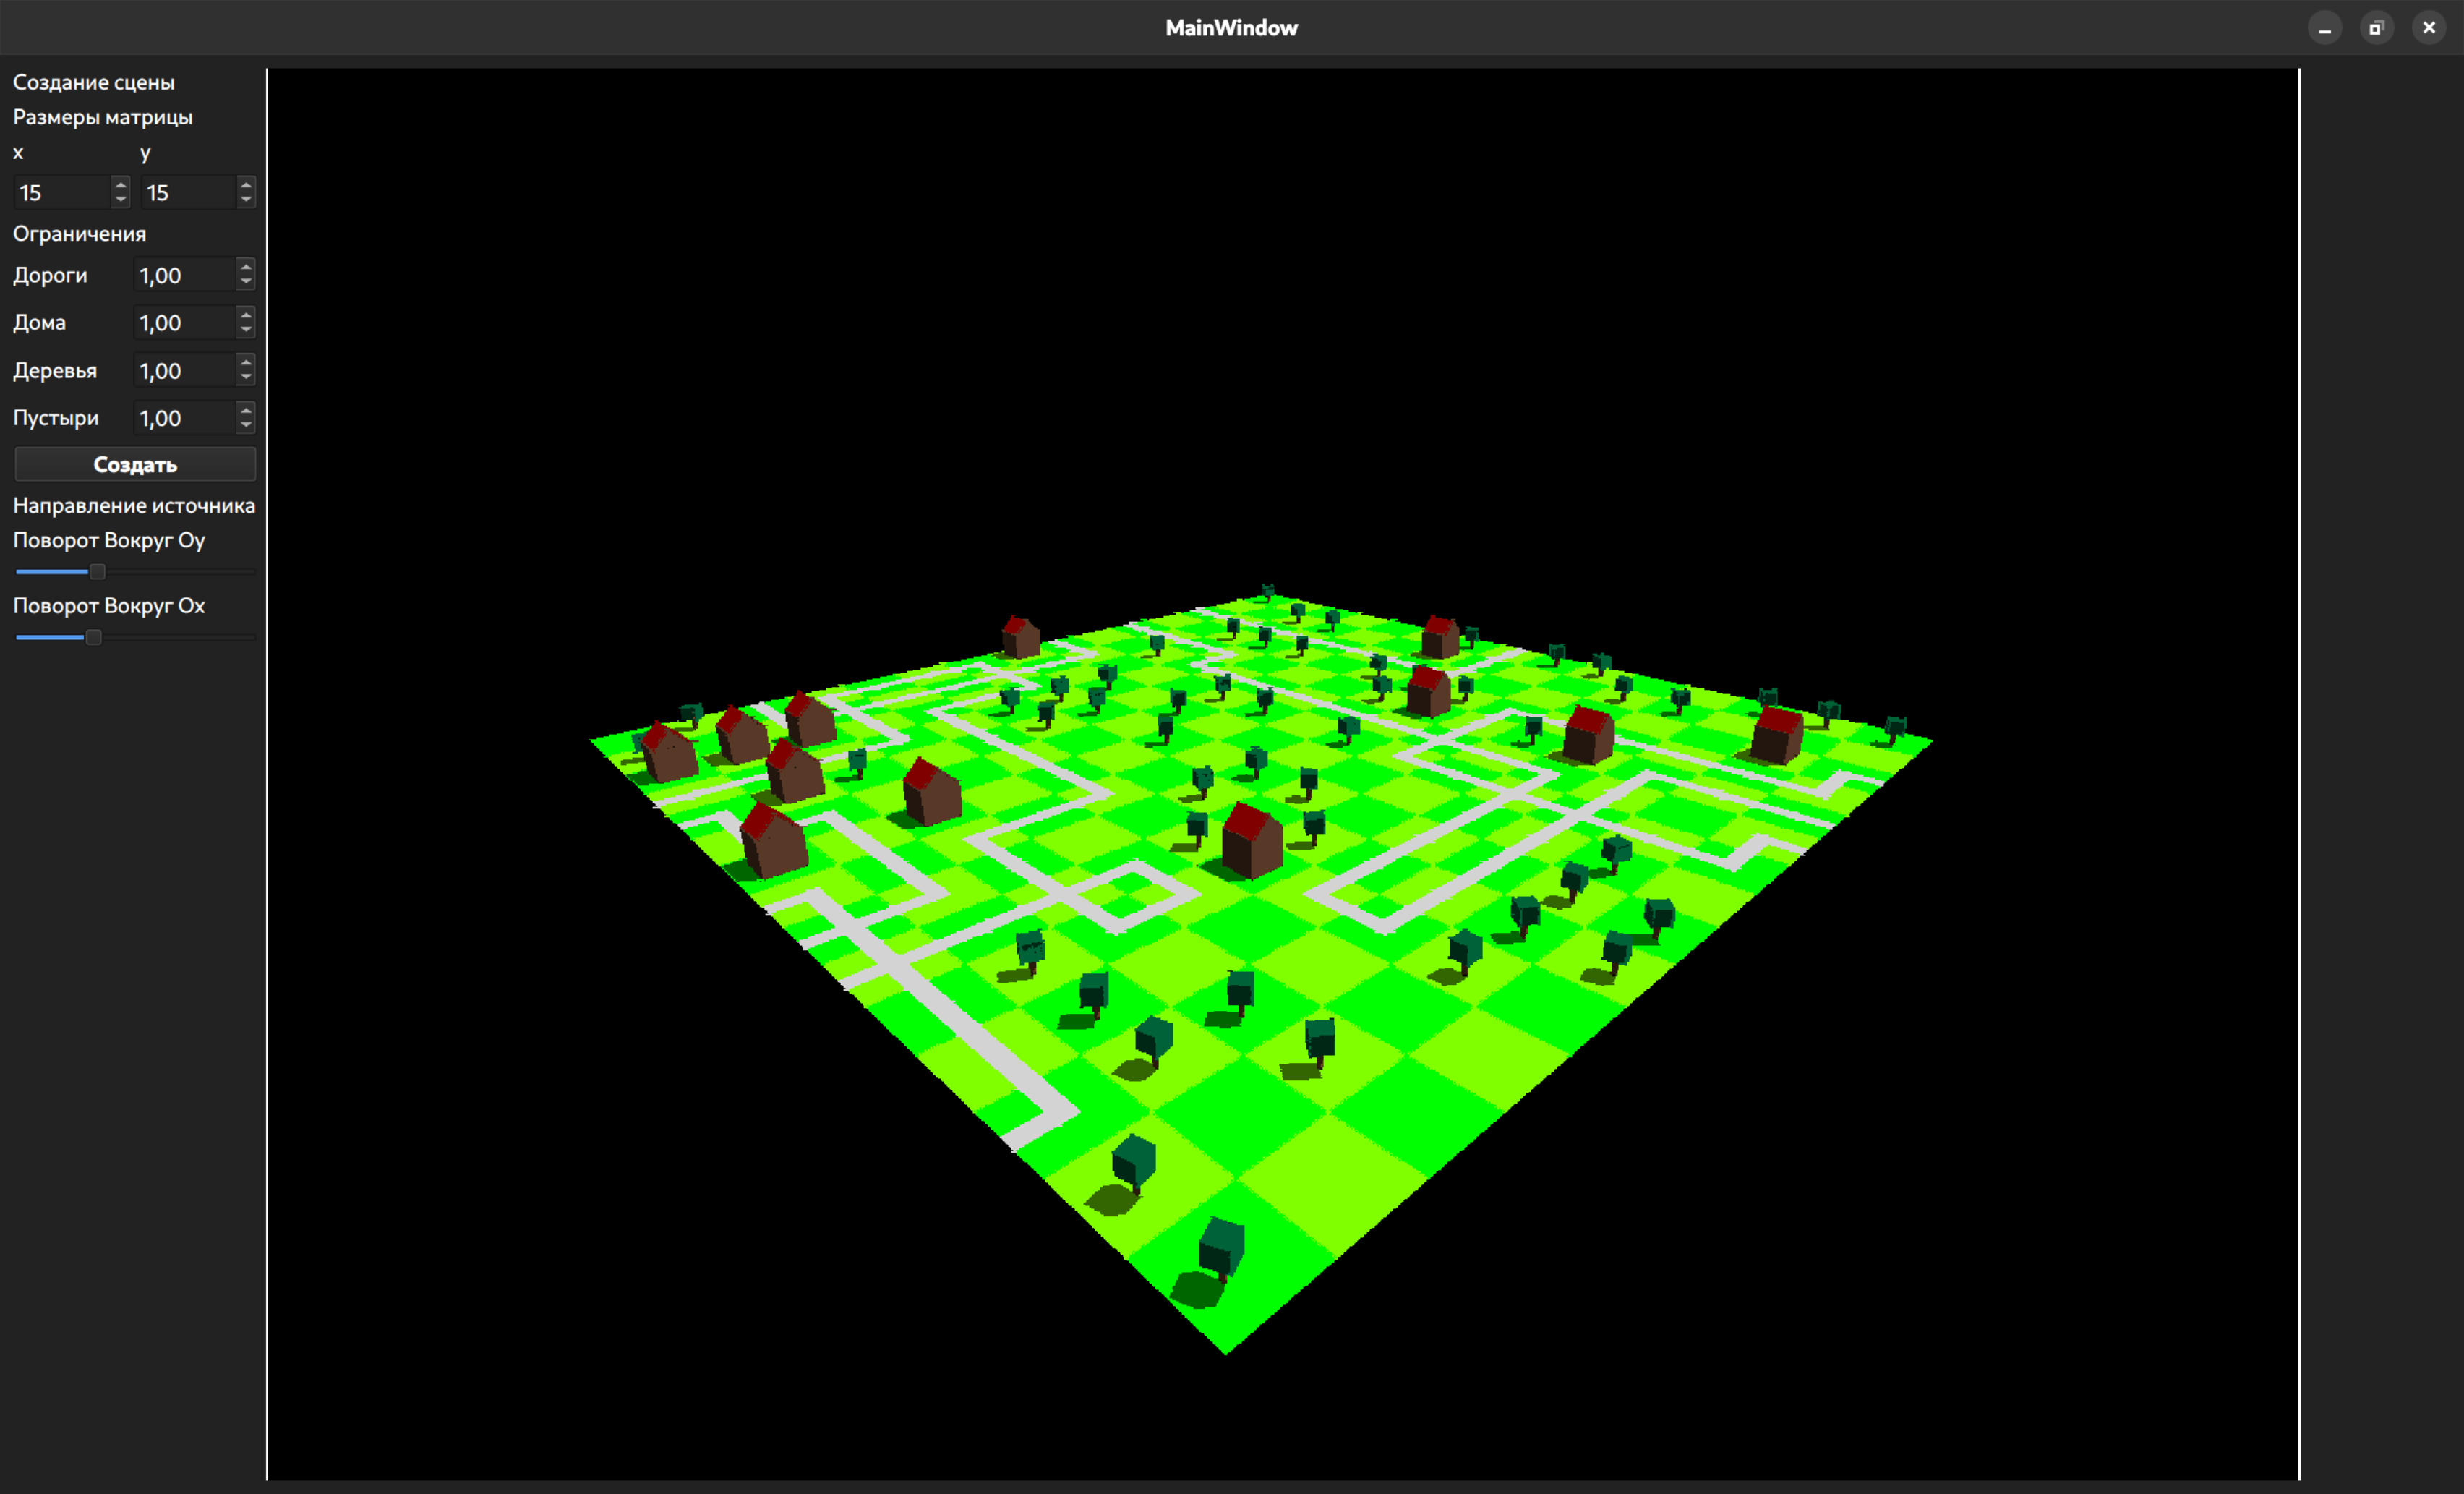
\includegraphics[width=\textwidth]{pic1}
  \caption{Пример работы программы --- генерация посёлка 15 на 15 ячеек}
  \label{fig:example_1}
\end{figure}
\begin{figure}[h!]
  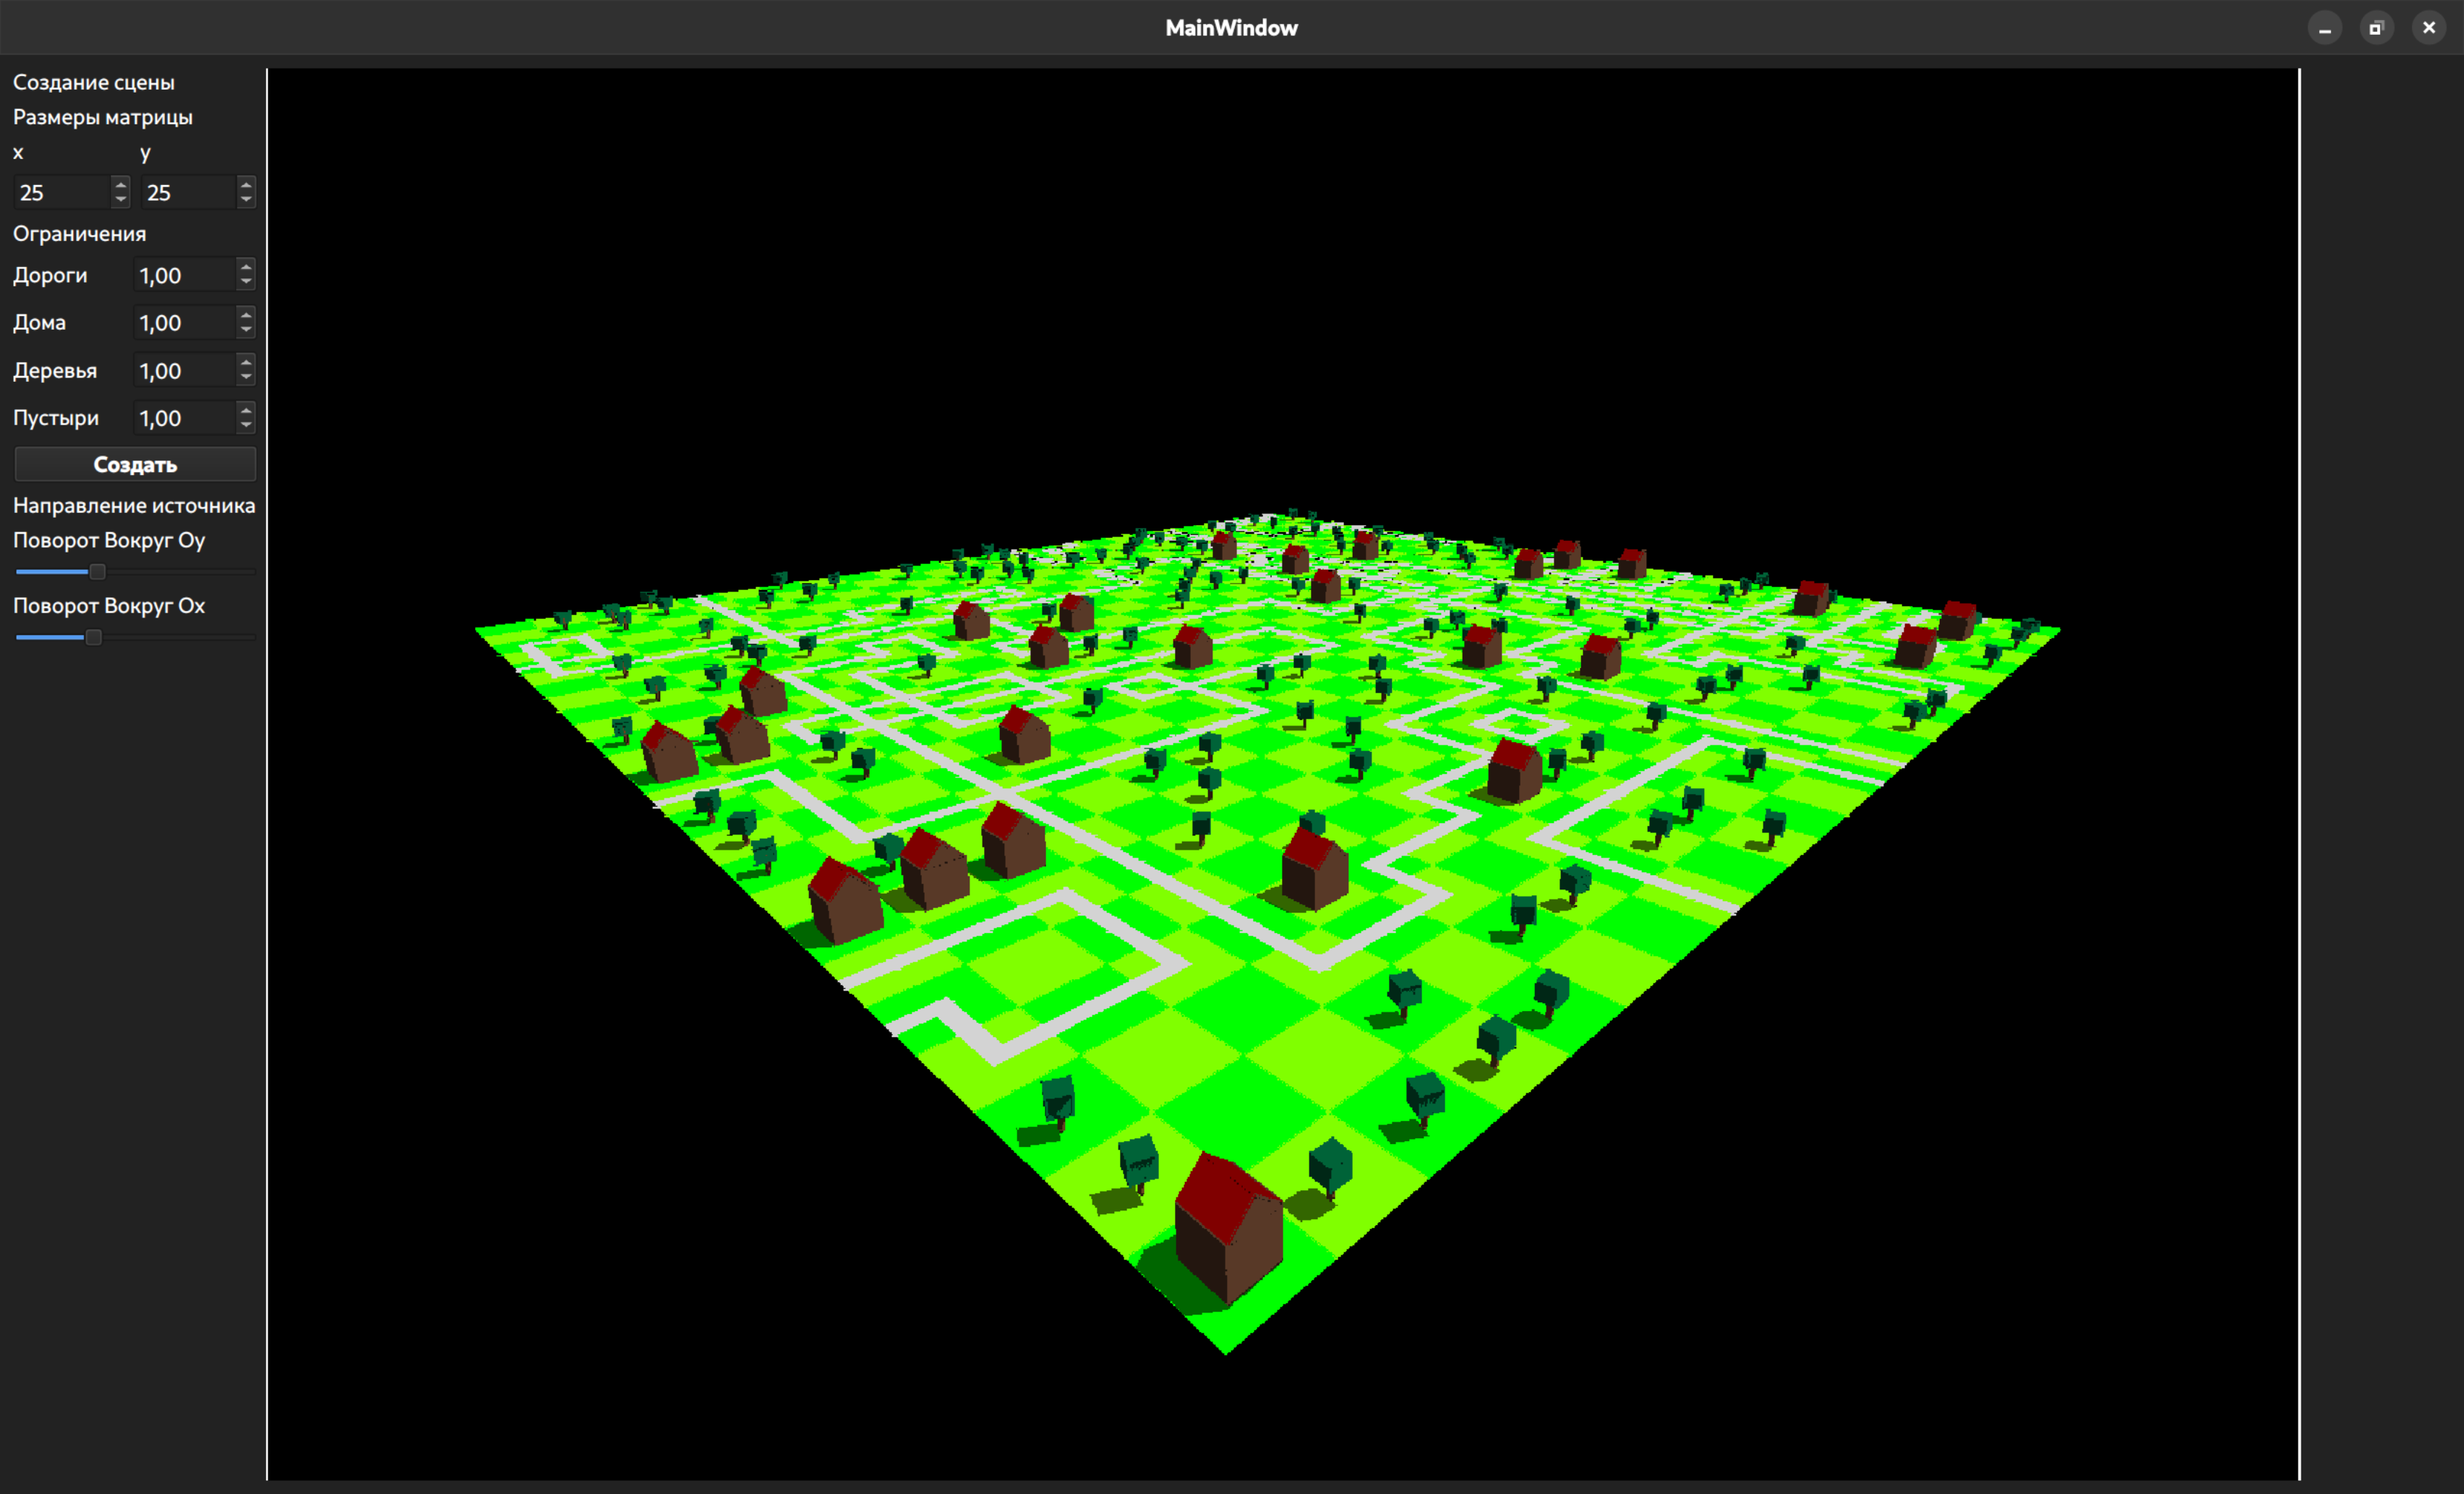
\includegraphics[width=\textwidth]{pic2}
  \caption{Пример работы программы ---  генерация посёлка 25 на 25 ячеек}
  \label{fig:example_2}
\end{figure}
\begin{figure}[h!]
  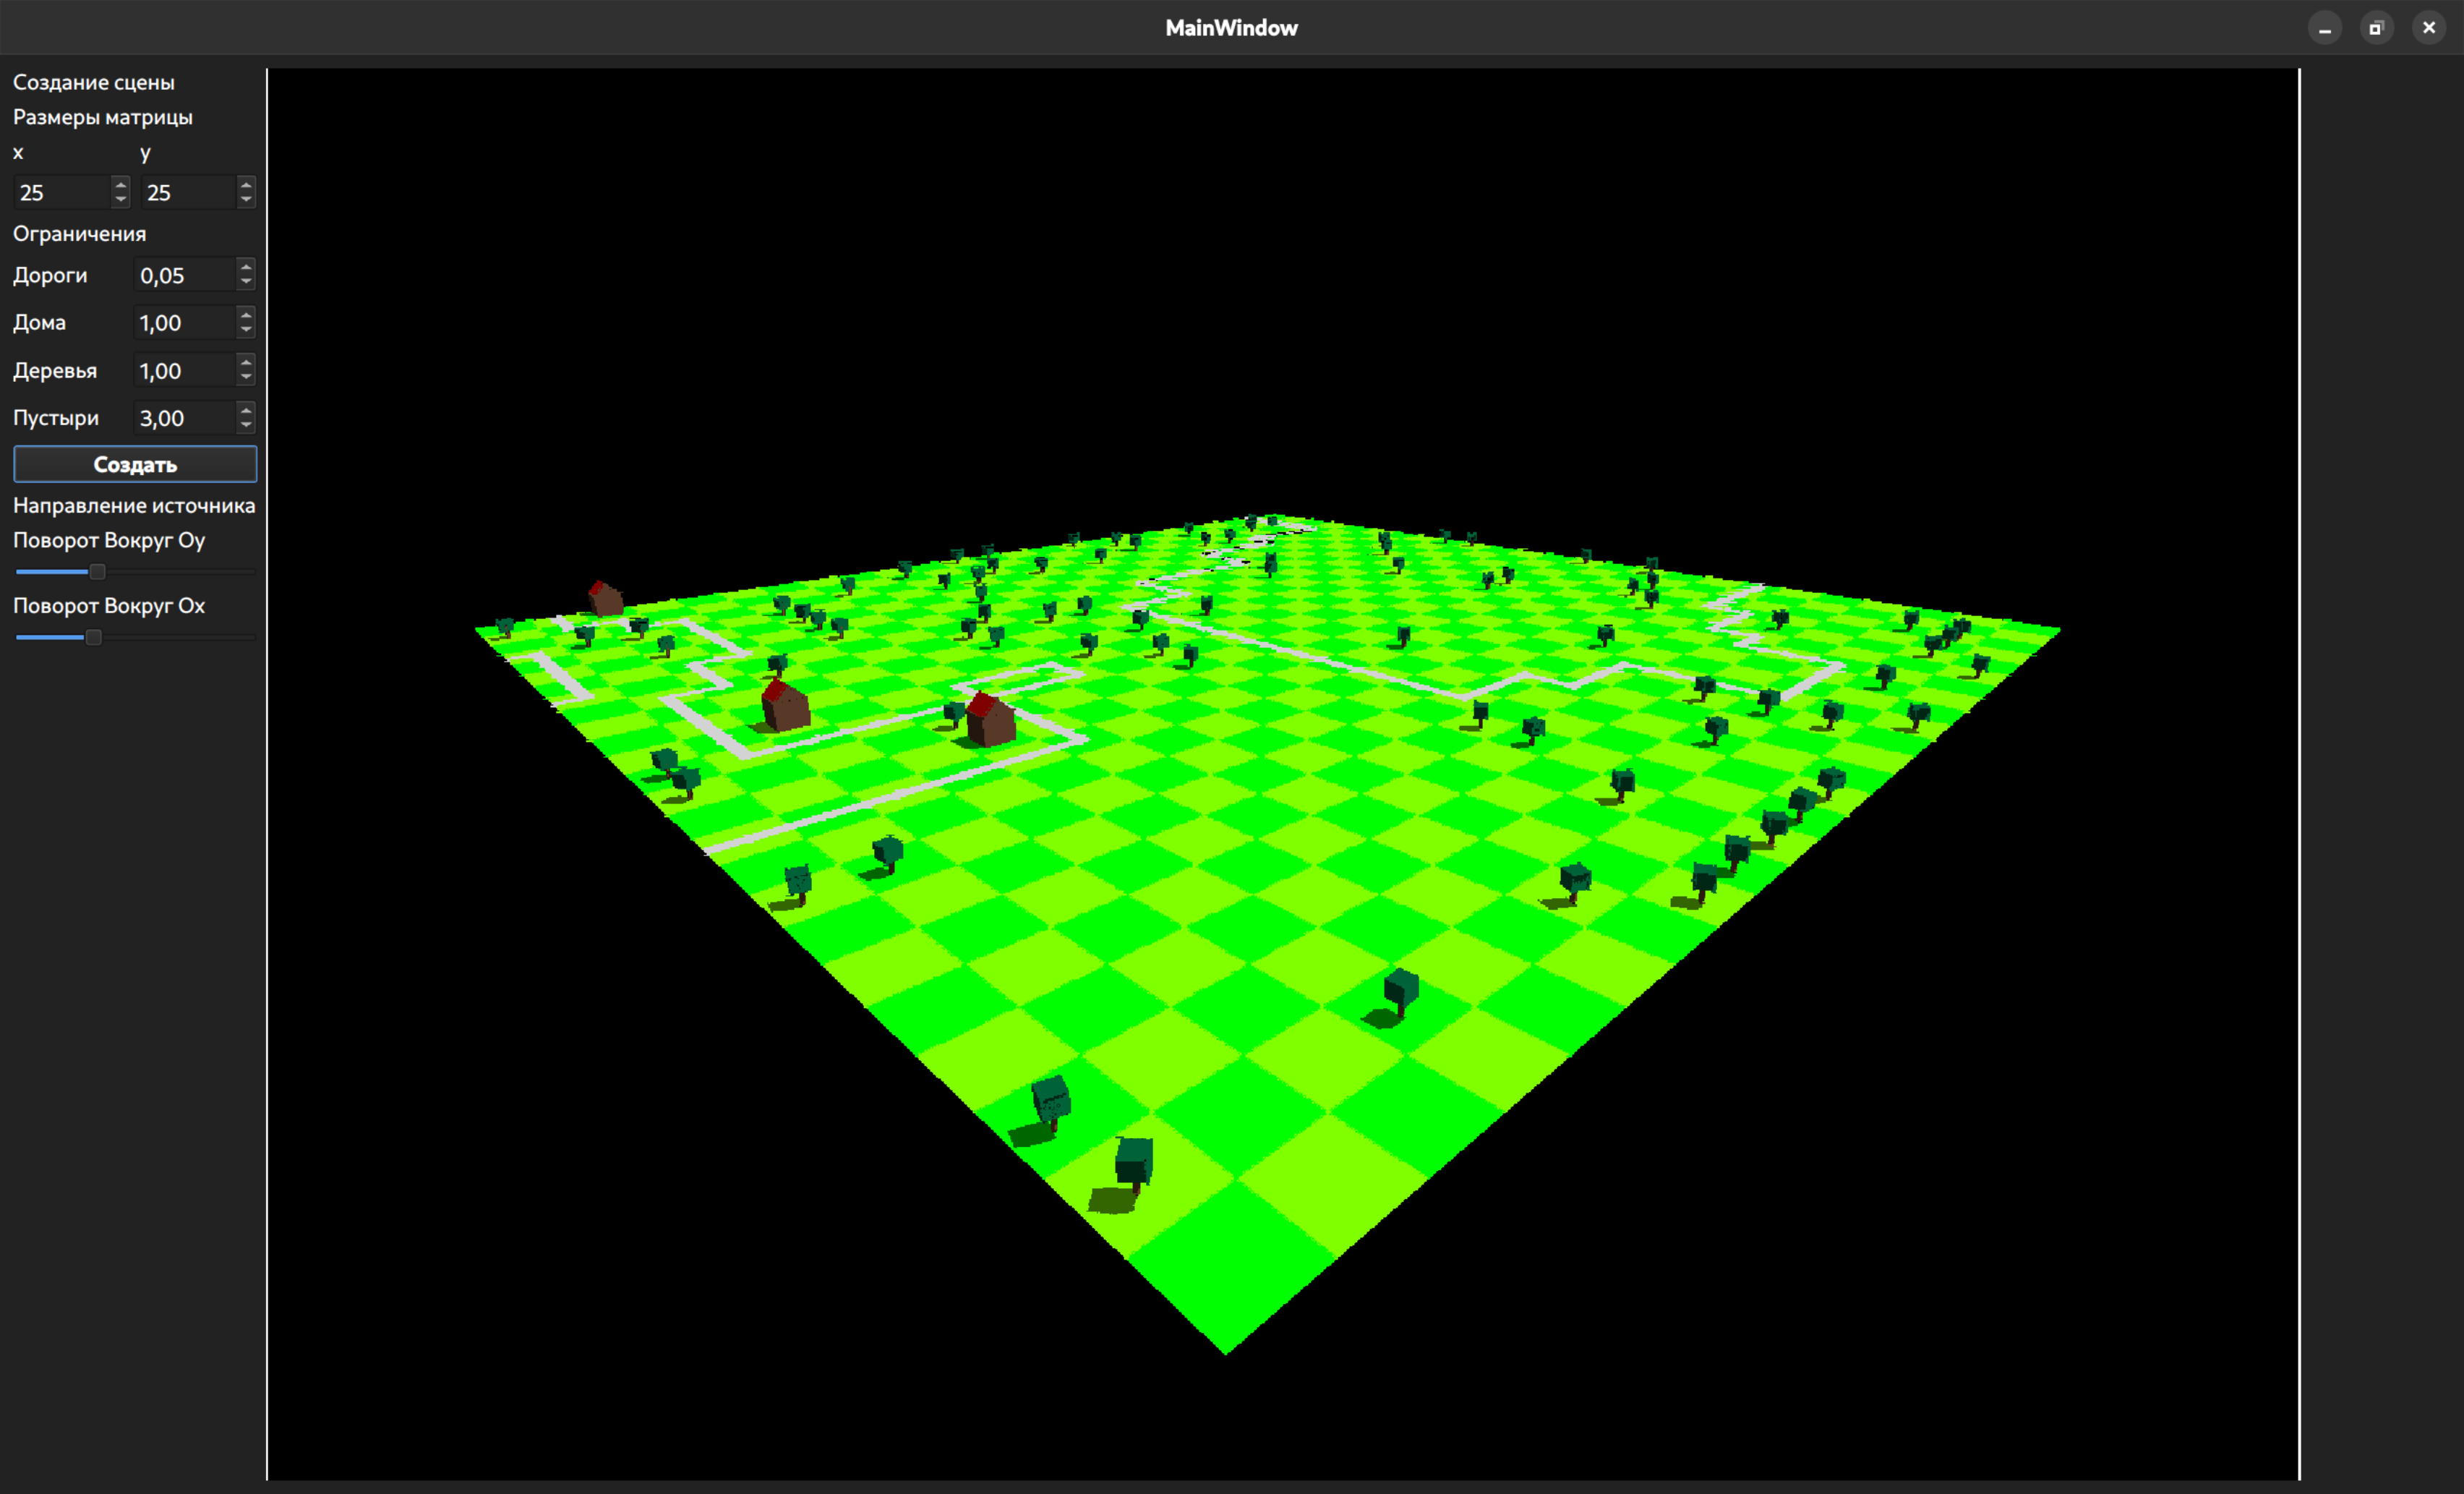
\includegraphics[width=\textwidth]{pic3}
  \caption{Пример работы программы --- генерация посёлка с уменьшенным количеством дорог и увеличенным колчичеством пустырей}
  \label{fig:example_3}
\end{figure}
\begin{figure}[h!]
  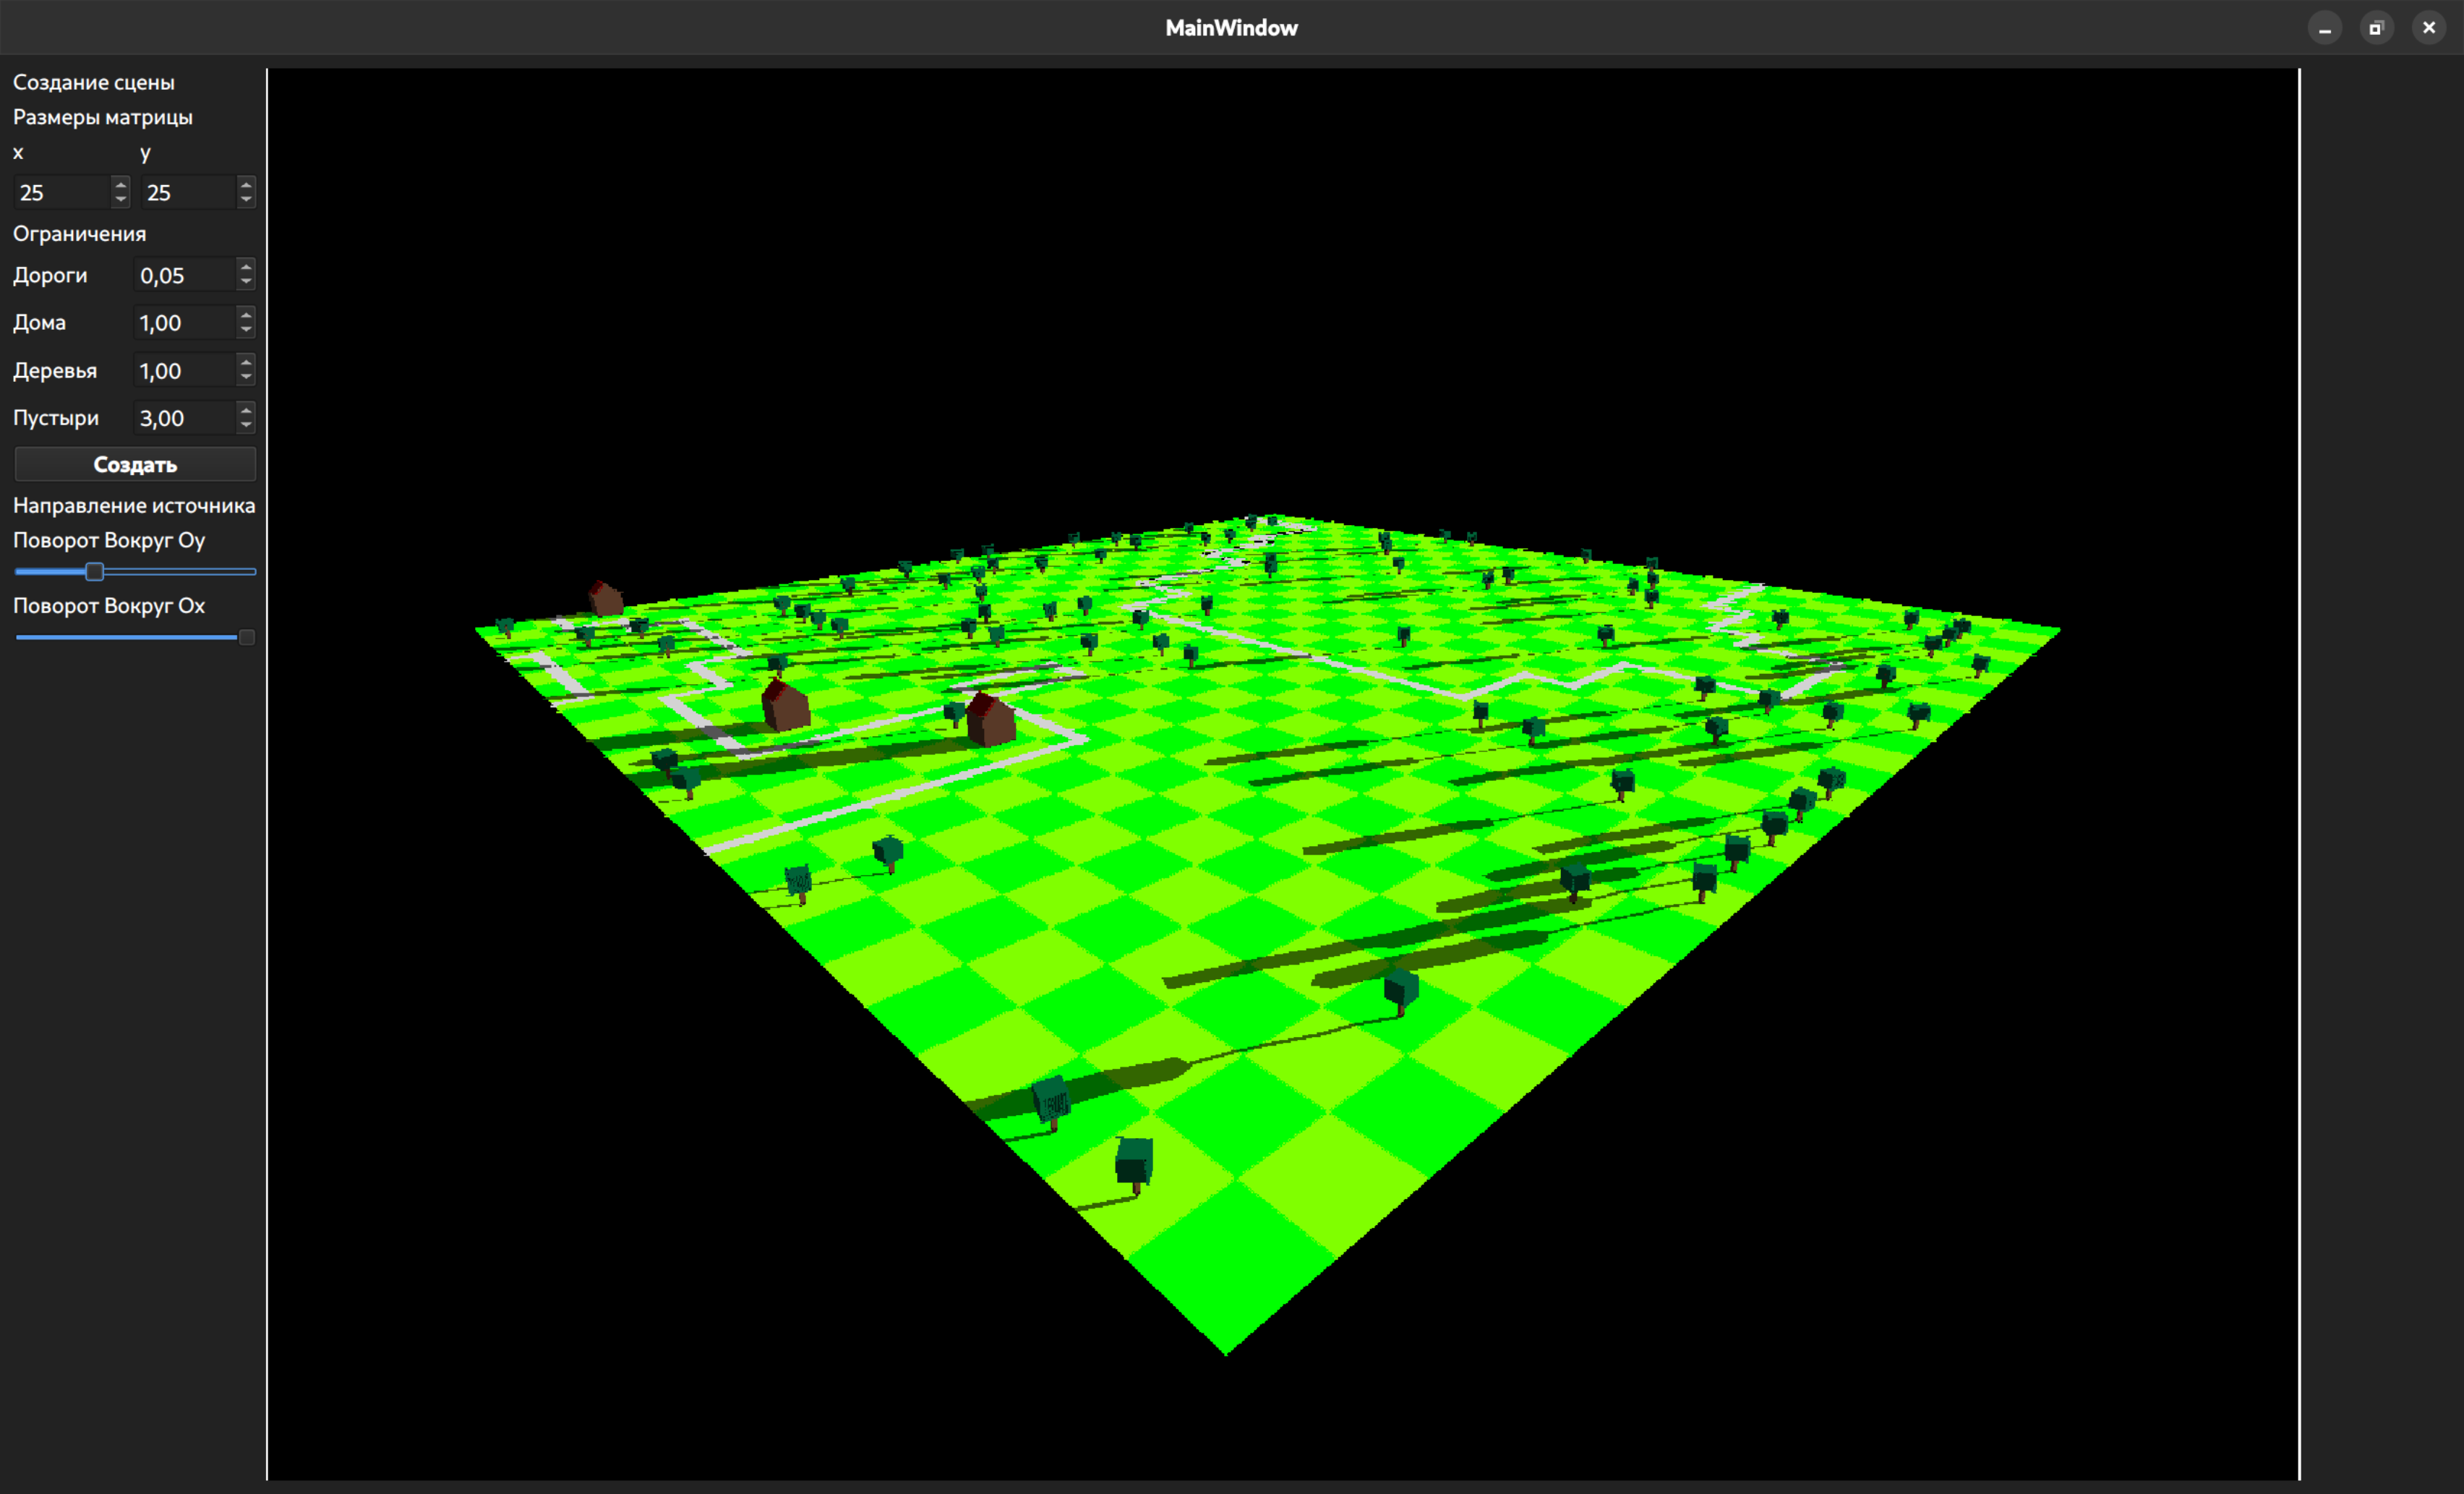
\includegraphics[width=\textwidth]{pic4}
  \caption{Пример работы программы --- Источник света приближен к земле, тени становятся длиннее}
  \label{fig:example_4}
\end{figure}
\begin{figure}[h!]
  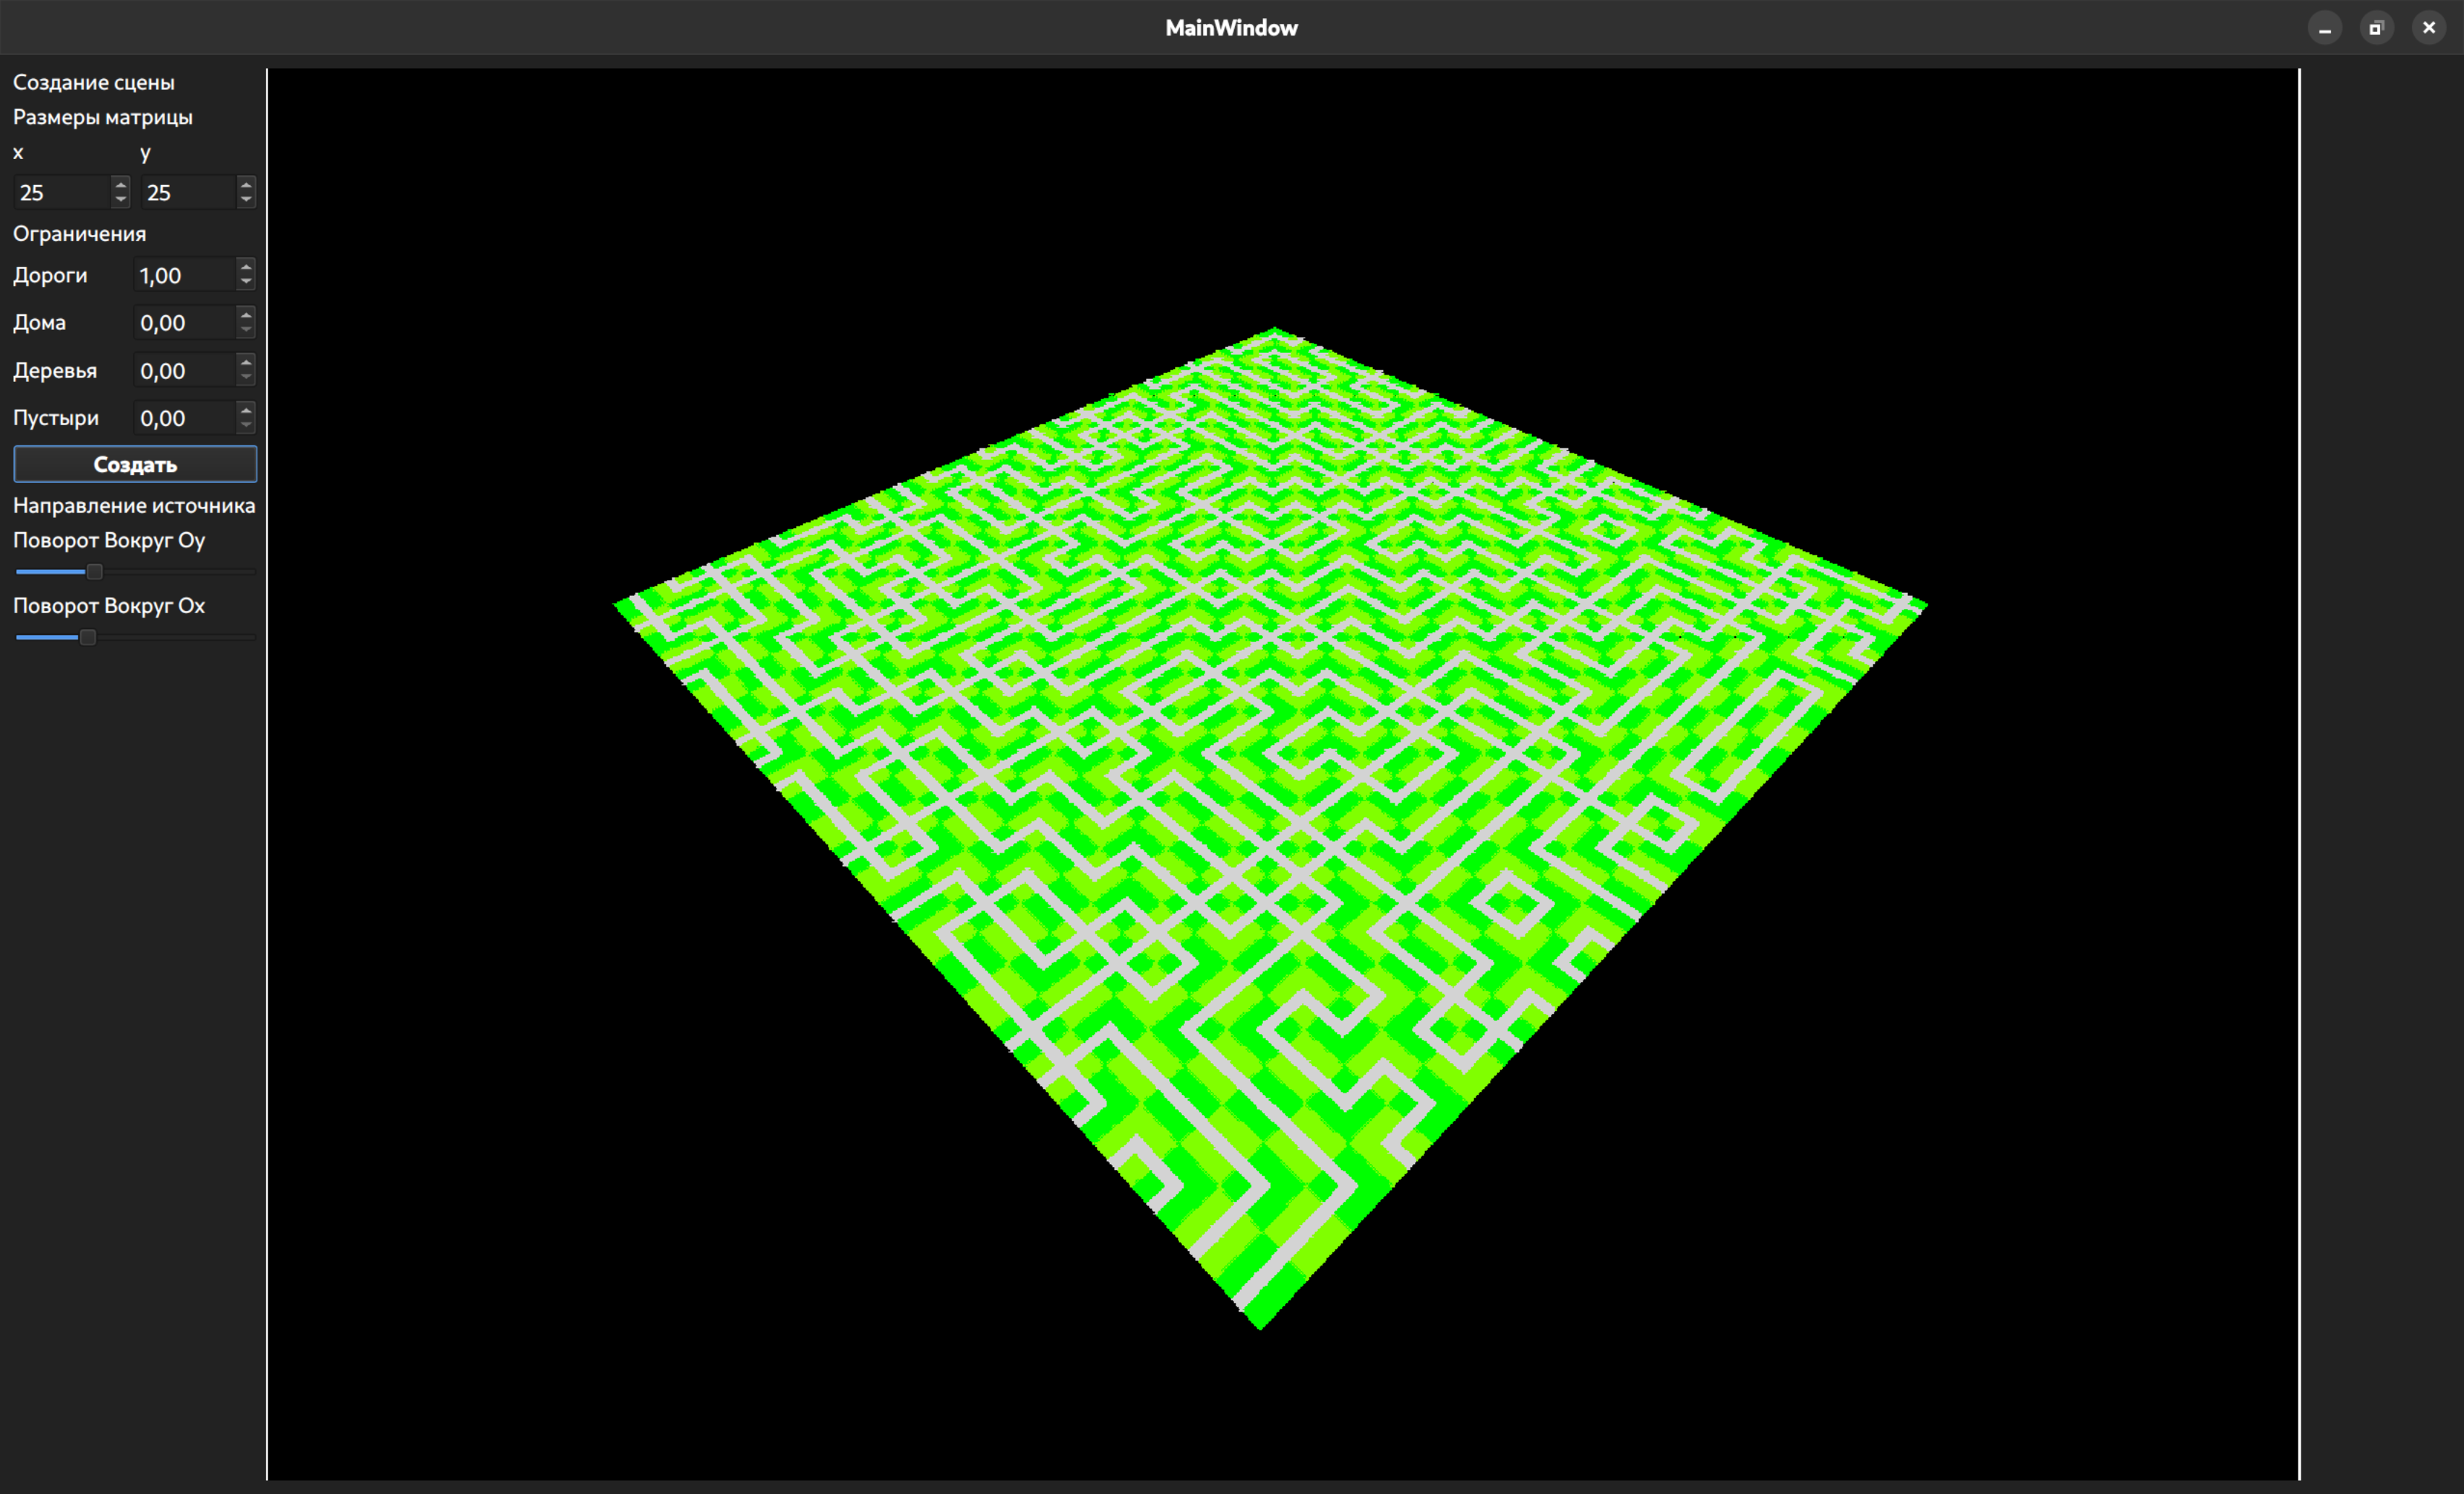
\includegraphics[width=\textwidth]{pic5}
  \caption{Пример работы программы --- запрещено появление любых объектов кроме дорог}
  \label{fig:example_5}
\end{figure}

\newpage

\

\section{Вывод}

Была осуществлена реализация программного обеспечения для создания конструирования и визуализации загородного посёлка.

\chapter{Исследовательская часть}

\section{Технические характеристики}

Технические характеристики устройства, на котором выполнялось исследование:
\begin{itemize}
  \item операционная система EndeavourOS 64бит;
  \item версия ядра Linux Linux 6.12.3-arch1-1;
  \item 13th Gen Intel(R) Core(TM) i5-13500H 4.70 ГГц 12 ядер (4
  производительных + 8 энергоэффективных) 16 логических процессоров;
  \item оперативная память 16ГБ с частотой 5200МГц.
\end{itemize}

\section{Описание исследования}

Было произведено несколько исследований.

\subsection*{Исследование времени генерации сцены}

Было проведено исследования времени генерации сцены от размеров матрицы. В ходе исследования производилась генерация квадратных сцен.

Для каждого размера матрицы, замер времени проводился 10 раз. В качестве результата сохранялось среднее значение затраченного времени.

Для замеров времени использовалась библиотека chrono, являющаяся частью стандартной библиотеки языка c++~\cite{cpp}.

Результаты временных замеров представлены в виде графика на рисунке~\ref{fig:qwfc_graph}.

\begin{figure}[h!]
  \centering
  \includesvg[width=.7\textwidth]{qwfcprof.svg}
  \caption{График зависимости времени генерации сцены от размеров сцены}
  \label{fig:qwfc_graph}
\end{figure}

\subsection*{Исследование времени создания карты теней}

Было проведено исследования зависимости времени создания карты теней от размеров буфера глубины. Размеры буфера по оси $Ox$ и $Oy$ в процессе исследования совпадали, то есть буфер был квадратным.

Количество моделей на сцене во время временных замеров оставалось постоянным.

Для замеров времени использовалась библиотека chrono, являющаяся частью стандартной библиотеки языка c++~\cite{cpp}.

Результаты временных замеров представлены в виде графика на рисунке~\ref{fig:smap_graph}.

\begin{figure}[h!]
  \centering
  \includesvg[width=.7\textwidth]{smapprof.svg}
  \caption{График зависимости времени создания карты теней от её разрешения}
  \label{fig:smap_graph}
\end{figure}

\subsection*{Исследование времени генерации кадра}

Было проведено исследования зависимости времени генерации от размеров матрицы сцены. В процессе исследования рассматривались только квадратные сцены.

Разрешение экрана (то есть размеры буфера кадра) в процессе исследования оставались постоянными.

Для замеров времени использовалась библиотека chrono, являющаяся частью стандартной библиотеки языка c++~\cite{cpp}.

Результаты временных замеров представлены в виде графика на рисунке~\ref{fig:render_graph}.

\begin{figure}[h!]
  \centering
  \includesvg[width=.7\textwidth]{rendprof.svg}
  \caption{График зависимости времени генерации кадра от размеров сцены}
  \label{fig:render_graph}
\end{figure}

\newpage

\section{Вывод}

Проанализировав графики, можно увидеть, что:
\begin{itemize}
  \item зависимость времени генерации квадратной сцены от размера стороны матрицы близка к степенной функции; 
  \item зависимость времени создания квадратной карты теней от размера стороны её буфера глубины близка к степенной функции; 
  \item зависимость времени генерации кадра от размера сцены (а соответственно и количества объектов на ней) близка к линейной.
\end{itemize}


\ssr{ЗАКЛЮЧЕНИЕ}

Поставленная цель была достигнута, и были выполнены все поставленные задачи:
\begin{itemize}
  \item были сравнены существующие алгоритмы процедурной генерации сцены и алгоритмы компьютерной графики, использующихся для визуализации трёхмерной модели (сцены);
  \item были выбраны подходящие алгоритмы для решения поставленных задач;
  \item были спроектированы архитектура и графический интерфейс ПО
  \item были выбраны средства реализации ПО;
  \item было разработано спроектированное ПО;
  \item были проведены замеры временных характеристик разработанного ПО.
\end{itemize}

В ходе проведенного исследования была проанализирована зависимость времени генерации квадратной сцены от размера стороны матрицы. Эта зависимость оказалась близка к степенной функции.

В ходе проведенного исследования была проанализирована зависимость времени создания квадратной карты теней от размера стороны её буфера глубины. Эта зависимость оказалась близка к степенной функции.

В ходе проведенного исследования была проанализирована зависимость времени генерации кадра от размера сцены (а соответственно и количества объектов на ней). Эта зависимость оказалась близка к линейной.


\def\bibname{\begin{center}\Large СПИСОК ИСПОЛЬЗОВАННЫХ ИСТОЧНИКОВ\end{center}}

\addcontentsline{toc}{chapter}{СПИСОК ИСПОЛЬЗОВАННЫХ ИСТОЧНИКОВ}
\begin{thebibliography}{}
  \bibitem{CGPaP} John F. Hugens. Computer Graphics Principles and Practice // 3-е издание // Бостон: Addison Wesley Professional // 1263 страницы

  \bibitem{QWFC} Heese, Raoul. Quantum Wave Function Collapse for Procedural Content Generation // статья // Institute of Electrical and Electronics Engineers (IEEE) // 13 страниц

  \bibitem{Rogers} Д. Роджерс Алгоритмические основы машинной графики // Перевод С.А. Вичес // Москва: Мир 1989г. // 512 страниц 

  \bibitem{Shadows} А.В. Мальцев Моделирование теней в 3D сценах с помощью каскадных теневых карт в режиме реального времени // статья // Журнал ИНФОРМАЦИОННЫЕ ТЕХНОЛОГИИ И ВЫЧИСЛИТЕЛЬНЫЕ СИСТЕМЫ // Москва: Российская Академия Наук 2014г. // 52 страницы

  \bibitem{LightMaps} Michael Abrash. Quake's lighting model: Surface caching. // Онлайн-ресурс: https://www.bluesnews.com/abrash/chap68.shtml // дата обращения: 03.11.2004

  % \bibitem{python3-matplotlib} Документация библиотеки Matplotlib: Visualization with Python /  [Электронный ресурс] // Matplotlib : [сайт]. — URL: https://matplotlib.org/ (дата обращения: 25.09.2024).

  % \bibitem{itmo-levenstein} Романовский И.В. Дискретный : Учебное пособие для студентов, специализирующихся по прикладной маткматике и информатике. // 4-е издание, исправленное и дополненное. // СПб.: Невский диалект; БХВ-Петербург, 2008. // 336 страниц

\end{thebibliography}

\renewcommand\thechapter{A}

\ssr{ПРИЛОЖЕНИЕ A}

\begin{lstlisting}[caption={Использование RenderVisitor на сцену}, label={lst:render_scene}]
void RenderVisitor::visit(Scene &ref) {
  ShadowMap &smap = Singleton<ShadowMap>::instance();
  auto resolution = ctx->getResolution();
  colors.resize(resolution.second, std::vector<Color>(resolution.first));
  depth.resize(resolution.second,
               std::vector<double>(resolution.first,
                                   std::numeric_limits<double>::infinity()));
  pixmaps.clear();

  tbb::parallel_for_each(ref.begin(), ref.end(), [this](const auto &newref) {
    newref.second->accept(*this);
  });

  for (const MyPixmap &pmap :
       pixmaps | std::views::filter([](const MyPixmap &pmap) {
         return !pmap.getDepth().empty() && !pmap.getDepth().front().empty();
       })) {
    auto &pdepth = pmap.getDepth(); auto offset = pmap.getOffset();
    auto &pcolor = pmap.getColor(); auto &pbright = pmap.getBrightness();

    for (int x = 0; x < pdepth.front().size(); ++x)
      for (int y = 0; y < pdepth.size(); ++y) {
        if (pdepth[y][x] < depth[y + offset.second][x + offset.first]) {
          depth[y + offset.second][x + offset.first] = pdepth[y][x];
          if (smap.isValid())
            colors[y + offset.second][x + offset.first] =
                pcolor * pbright[y][x];
          else
            colors[y + offset.second][x + offset.first] = pcolor;
        }
      }
  }

  ctx->setImage(colors);
}
\end{lstlisting}

\begin{lstlisting}[caption={Использование RenderVisitor на модель}, label={lst:render_model}]
void RenderVisitor::visit(FaceModel &ref) {
  ShadowMap &smap = Singleton<ShadowMap>::instance();

  std::shared_ptr<TransformationMatrix> transf = ref.getTransformation();

  CameraManager &cm = Singleton<CameraManager>::instance();

  std::shared_ptr<BaseCamera> cam =
      std::dynamic_pointer_cast<BaseCamera>(cm.getCamera());
  std::shared_ptr<TransformationMatrix> camtransf = cam->getTransformation();

  PTSCAdapter->setCamera(cm.getCamera());
  Point3D cam_position = cam->getPosition();
  auto resolution = ctx->getResolution();

  auto range =
      ref.getFaces() |
    std::views::filter(std::bind(&Face::isVisible, std::placeholders::_1,
                                    cam_position, *transf)) |
      std::views::filter([&transf, &camtransf](const Face &f) {
        return std::ranges::any_of(f.getPoints(), [&transf, &camtransf](
                                                      const Point3D &pt) {
    return camtransf->apply(transf->apply(pt)).z >= 2 * MyMath::EPS;
        });
      });

  tbb::parallel_for_each(
      range.begin(), range.end(),
      [this, &camtransf, &transf, &resolution, &smap](const Face &face) {
        pixmaps.emplace_back(face.getPixmap(
            [transf](const Point3D &pt) { return transf->apply(pt); },
            [&camtransf](const Point3D &pt) { return camtransf->apply(pt); },
            [this, &smap](const Point3D &pt) {
              return PTSCAdapter->convert(pt);
            },
            resolution.first, resolution.second, smap, true));
      });
}  
\end{lstlisting}

\iffalse
\begin{lstlisting}[caption={Растеризация треугольника --- начало}, label={lst:render_triangle}]
MyPixmap Triangle::getPixmap(
    std::function<Point3D(const Point3D &)> to_world,
    std::function<Point3D(const Point3D &)> to_camera,
    std::function<std::shared_ptr<Point2D>(const Point3D &)> to_screen,
    size_t screen_width, size_t screen_height, const Color &color,
    const ShadowMap &smap, bool center_axis) const {
  int centerX = center_axis ? static_cast<int>(screen_width / 2) : 0;
  int centerY = center_axis ? static_cast<int>(screen_height / 2) : 0;

  Point3D t0 = to_world(p1); 
  Point3D t1 = to_world(p2); 
  Point3D t2 = to_world(p3);

  Point3D v0 = to_camera(t0); 
  Point3D v1 = to_camera(t1); 
  Point3D v2 = to_camera(t2);

  std::shared_ptr<Point2D> pt1_screen = to_screen(v0);
  std::shared_ptr<Point2D> pt2_screen = to_screen(v1);
  std::shared_ptr<Point2D> pt3_screen = to_screen(v2);

  Point2D p0_2d(pt1_screen->x + centerX, pt1_screen->y + centerY);
  Point2D p1_2d(pt2_screen->x + centerX, pt2_screen->y + centerY);
  Point2D p2_2d(pt3_screen->x + centerX, pt3_screen->y + centerY);

  if (p1_2d.y < p0_2d.y) {
    std::swap(p0_2d, p1_2d); std::swap(v0, v1); std::swap(t0, t1);
  }
  if (p2_2d.y < p1_2d.y) {
    std::swap(p1_2d, p2_2d); std::swap(v1, v2); std::swap(t1, t2);
  }
  if (p1_2d.y < p0_2d.y) {
    std::swap(p0_2d, p1_2d); std::swap(v0, v1); std::swap(t0, t1);
  }

  auto interpolate = [](double y1, double x1, double y2, double x2, double y) {
    if (y1 == y2) return x1;
    return x1 + (x2 - x1) * (y - y1) / (y2 - y1);
  };
\end{lstlisting}
\begin{lstlisting}[caption={Продолжение Растеризация треугольника}, label={lst:render_triangle1}]
  auto interpolateZ = [](double y1, double z1, double y2, double z2, double y) {
    if (y1 == y2) return z1;
    return z1 + (z2 - z1) * (y - y1) / (y2 - y1);
  };

  auto interpolatePart = [](double v1, double v2, int y1, int y2, int y) {
    return v1 + (v2 - v1) * (y - y1) / static_cast<double>(y2 - y1);
  };

  auto interpolatePoint = [&interpolatePart](const Point3D &p1,
                                             const Point3D &p2, int y1, int y2,
                                             int y) {
    return Point3D(interpolatePart(p1.x, p2.x, y1, y2, y),
                   interpolatePart(p1.y, p2.y, y1, y2, y),
                   interpolatePart(p1.z, p2.z, y1, y2, y));
  };

  int minY = std::max(0, static_cast<int>(std::floor(p0_2d.y)));
  int minYClamped = std::clamp(minY, 0, static_cast<int>(screen_height));
  int maxY = std::min(static_cast<int>(screen_height),
               static_cast<int>(std::ceil(p2_2d.y))) + 1; 
  int maxYClamped = std::clamp(maxY, 0, static_cast<int>(screen_height));

  int minX = std::min({static_cast<int>(p0_2d.x),
                       static_cast<int>(p1_2d.x),
                       static_cast<int>(p2_2d.x)});
  int minXClamped = std::clamp(minX, 0, static_cast<int>(screen_width));
  int maxX = std::max({static_cast<int>(p0_2d.x),
                static_cast<int>(p1_2d.x),
                static_cast<int>(p2_2d.x)}) + 1;
  int maxXClamped = std::clamp(maxX, 0, static_cast<int>(screen_width));

  if (maxXClamped - minXClamped <= 0 || maxYClamped - minYClamped <= 0)
    return MyPixmap(0, 0);

  MyPixmap res(maxXClamped - minXClamped, maxYClamped - minYClamped,
               minXClamped, minYClamped, smap.isValid());
\end{lstlisting}

\begin{lstlisting}[caption={Продолжение Растеризация треугольника}, label={lst:render_triangle2}]
  std::vector<std::vector<double>> &depth = res.getDepthE();
  std::vector<std::vector<double>> &brightness = res.getBrightnessE();
  res.setColor(color);

  for (int y = minYClamped; y < maxYClamped; ++y) {
    double xLeft, xRight, zLeft, zRight;
    Point3D worldLeft, worldRight;

    if (y < p1_2d.y) {
      xLeft = interpolate(p0_2d.y, p0_2d.x, p1_2d.y, p1_2d.x, y);
      xRight = interpolate(p0_2d.y, p0_2d.x, p2_2d.y, p2_2d.x, y);
      zLeft = interpolateZ(p0_2d.y, v0.z, p1_2d.y, v1.z, y);
      zRight = interpolateZ(p0_2d.y, v0.z, p2_2d.y, v2.z, y);

      worldLeft = interpolatePoint(t0, t1, p0_2d.y, p1_2d.y, y);
      worldRight = interpolatePoint(t0, t2, p0_2d.y, p2_2d.y, y);
    } else {
      xLeft = interpolate(p1_2d.y, p1_2d.x, p2_2d.y, p2_2d.x, y);
      xRight = interpolate(p0_2d.y, p0_2d.x, p2_2d.y, p2_2d.x, y);
      zLeft = interpolateZ(p1_2d.y, v1.z, p2_2d.y, v2.z, y);
      zRight = interpolateZ(p0_2d.y, v0.z, p2_2d.y, v2.z, y);

      worldLeft = interpolatePoint(t1, t2, p1_2d.y, p2_2d.y, y);
      worldRight = interpolatePoint(t0, t2, p0_2d.y, p2_2d.y, y);
    }

    if (xLeft > xRight) {
      std::swap(xLeft, xRight);
      std::swap(zLeft, zRight);
      std::swap(worldLeft, worldRight);
    }

int xStart = std::max(minXClamped, static_cast<int>(std::floor(xLeft)));
int xEnd = std::min(maxXClamped, static_cast<int>(std::ceil(xRight) +1.));

    if (xEnd - xStart <= 1)
      continue;
\end{lstlisting}
\newpage
\begin{lstlisting}[caption={Продолжение Растеризация треугольника}, label={lst:render_triangle3}]
    double z = zLeft;
    double dz = (xEnd >= xStart) ? (zRight - zLeft) / (xRight - xLeft) : 0;

    Point3D world = worldLeft;
    Point3D d_world = (xEnd > xStart)
                          ? (worldRight - worldLeft) / (xRight - xLeft)
                          : Point3D();

    if (std::ceil(xLeft) < xStart) {
      z += dz * (xStart - xLeft);
      world += d_world * (xStart - xLeft);
    }

    for (int x = xStart; x < xEnd; ++x) {
      depth[y - minYClamped][x - minXClamped] = z;
      if (smap.isValid()) {
        brightness[y - minYClamped][x - minXClamped] =
            smap.getBrightness(world);
      }
      z += dz;
      world += d_world;
    }
  }

  return res;
}
\end{lstlisting}
\fi

\begin{lstlisting}[caption={Метод фиксирования состояния ячейки класса QWFC}, label={lst:qwfcoll}]
void QWFC::collapseCell(int x, int y) {
  if (x < 0 || y < 0 || x >= width || y >= height)
    return;
  auto &possibleValues = matrix[y][x];
  if (possibleValues.size() == 1)
    return;

  double totalProbability = 0.0;
  for (const auto &value : possibleValues) {
    totalProbability += cells.at(value).getProbability();
  }

  if (totalProbability < MyMath::EPS) {
    throw std::runtime_error("Can not continue.");
  }

  double random = static_cast<double>(rand()) / static_cast<double>(RAND_MAX) *
                  totalProbability;
  double cumulativeProbability = 0.0;
  int chosenValue = *possibleValues.begin();

  for (const auto &value : possibleValues) {
    cumulativeProbability += cells.at(value).getProbability();
    if (random <= cumulativeProbability) {
      chosenValue = value;
      break;
    }
  }

  possibleValues.clear();
  possibleValues.insert(chosenValue);
}
\end{lstlisting}

% \begin{lstlisting}[caption={}, label={lst:}]
% \end{lstlisting}
\newpage

\renewcommand\thechapter{B}

\ssr{ПРИЛОЖЕНИЕ B}

Презентация состоит из N слайдов.

\end{document}
